\chapter{Validations}
\label{chap:validation}

Dans les chapitres précédents, nous avons présenté la méthode
Galerkin Discontinue (GD)
et son implémentation parallèle optimisée pour traiter des mailles
hexaédriques. Nous avons aussi décrit plusieurs modèles physiques de
simulation et différents schémas d'intégration en temps.
\\

Dans ce dernier chapitre, nous présentons des résultats
permettant de valider notre implémentation de solveur GD, autant
par la précision des calculs que par leur vitesse d'exécution.

Ainsi, nous commençons par présenter des résultats de convergence
sur un cas académique de propagation d'une onde plane dans un cube.
Nous en profitons pour effectuer des comparaisons entre maillages
structurés (hexaèdres droits) et non structurés (issus du découpage de
tétraèdres).

Nous comparons ensuite notre solveur GD à un solveur implémentant
la méthode des différences finies sur un cas d'application
mettant en scène une antenne dipolaire à proximité de l'oreille d'une tête
humaine simplifiée. Nous donnons aussi les résultats, sur ce même cas d'application,
des différents schémas d'intégration en temps que nous avons présenté plus tôt.
Ce cas d'application s'apparente à une communication
téléphonique et a servi de fil conducteur au cours de cette thèse.

Le second fil conducteur a été l'objectif d'effectuer des simulations
sur un modèle de corps humain complet (avec organes) dans le cadre du projet HOROCH.
Nous présentons les résultats de la simulation effectuée sur ce modèle
de corps humain, à côté duquel nous avons placé
une antenne de type Bluetooth.
Il s'agit de la plus grande simulation réalisée par le solveur à ce jour.

Enfin, nous terminons par présenter les résultats d'efficacité du solveur
exécuté en parallèle sur un grand nombre de périphériques de calcul.
\\


\section{Simulation d'onde plane}
\label{sect:valid_onde_plane}

\subsection{Convergence du schéma couplé GD-RK2}
\label{ssect:cv_gd_rk2}


Pour déterminer l'ordre de convergence du schéma couplé GD-RK$2$, nous simulons la
propagation d'une onde plane dans le vide, à l'aide d'une surface de Huygens (section
\ref{sect:injection_ondes}).
La condition limite utilisée est le modèle de Silver-Müller
(section \ref{ssect:silver_mueller}).

Une onde plane est définie par une fonction donnant l'amplitude
du signal au cours du temps (proposition \ref{prop:onde_plane}).
Le signal que nous utilisons est une impulsion gaussienne définie sur
l'intervalle $\PbTps$ par :
\begin{align} \label{eq:onde_plane}
	t \mapsto A \exp \left( -\left( \frac{t - t_A}{\tau} \right)^2 \right) ,
\end{align}
avec $A$ l'amplitude de l'onde, 
$\tau$ donnant l'intervalle de temps entre les deux points de demie-amplitude
(de largeur $2 \sqrt{\ln 2} \tau$)
et $t_A$ l'antécédent de la valeur d'amplitude maximale
(figure \ref{img:onde_plane}).


\begin{figure}[!h]
	\begin{center}
		\caption{
			\label{img:onde_plane}
			Signal adimensionné définissant l'onde plane utilisée
			au cours des tests de convergence du schéma couplé GD-RK$2$.
		}
		
		\begin{tikzpicture}[scale=1]
		\begin{axis}[
		axis lines=middle,
		xlabel=$ct$, x label style={at={(axis cs:0.5,0)},anchor=north},
		ylabel=$0$, y label style={at={(axis cs:0,-0.05)},anchor=east},
		xmin=-0.05,xmax=0.5,ymin=-0.1,ymax=1.1,
		xtick={0,0.1,...,0.5},ytick={0,0.5,1},
		x post scale=1.5,
		y post scale=1.5,
		%legend style={at={(axis cs:0.9,0.2)},anchor=south west}
		]
		
		\addplot+[
		thick,
		mark=none,
		color=red,
		samples=200,
		domain=0:0.4
		]
		{exp(-((x-0.17953)/0.0683)^2)};
		
		\node[anchor=east] (a) at (axis cs:0.1227,0.5){};
		\node[anchor=west] (b) at (axis cs:0.2364,0.5){};
		\draw[arrows={latex-latex}](a)--node[midway,below]{$2 \sqrt{\ln 2} \tau$}(b);
		
		\node[anchor=east] (c) at (axis cs:0,1){};
		\node[anchor=west] (d) at (axis cs:0.17953,1){};
		\draw[dotted](c)--(d);
		
		\node[anchor=east] (e) at (axis cs:0,0.5){};
		\node[anchor=west] (f) at (axis cs:0.1227,0.5){};
		\draw[dotted](e)--(f);
		
		\node[anchor=north] (g) at (axis cs:0.17953,0){};
		\node[anchor=south] (h) at (axis cs:0.17953,1){};
		\draw[dotted](g)--(h);

		\node[anchor=south east] at (axis cs:0.17953,0){$t_A$};
		\node[anchor=north west] at (axis cs:0,1){$A$};
		
		\end{axis}
		\end{tikzpicture}
	\end{center}
\end{figure}



Afin de définir le signal temporel, nous utilisons la définition fréquentielle
de l'onde plane donnée par :
\begin{align}
\freq \mapsto
A \tau \sqrt{\pi} \exp \left( -(\pi \freq \tau)^2 - 2 j \pi \freq t_A \right) ,
\end{align}
avec $f$ la fréquence et $j$ le nombre complexe défini tel que $j^2 = -1$.
Nous pouvons alors définir notre signal en fonction de la fréquence maximale
$\freq_{\max}$ souhaitée
et retrouver le signal temporel grâce aux relations suivantes :
\begin{subequations}
	\begin{align}
		\tau &= \frac{\sqrt{- \ln (a_A)}}{\pi \freq_{\max}} ,
		\\
		t_A &= \tau \sqrt{- \ln (a_0)} ,
	\end{align}
\end{subequations}
où $a_0$ représente l'atténuation au temps initial ($t=0$)
et $a_A$ représente l'atténuation au temps d'amplitude maximale $t_A$.

Ces paramètres d'atténuation permettent de réduire la durée du signal.
Une impulsion gaussienne tend vers $0$ aux infinis, l'atténuation au temps
initial indique la tolérence à appliquer en $t=0$ afin de diminuer $t_A$ qui
est le retard permettant d'avoir le début de la gaussienne en temps positif.
L'atténuation au temps d'amplitude maximale permet de diminuer la valeur
de $\tau$ (\textit{i.e.} la durée de l'impulsion).
Pour notre cas d'application nous choisissons :
\begin{itemize}
	\item $A = 1$ ;
	\item $\freq_{\max} = 3$ GHz ;
	\item $a_0 = 0.001$ (ou $0.1$ \%).
	\item $a_A = 0.01$ (ou $1$ \%) ;
\end{itemize}
Avec ces valeurs, dans le cas adimensionné,
nous avons $\tau \approx 0.0683$ et $t_A \approx 0.1795$,
ce qui nous donne une durée de signal d'environ $1.2$ ns.

La direction de propagation choisie est suivant la composante $\x_3$.
Le champ $\E$ varie selon la composante $\x_1$ de l'espace et le champ
$\H$ varie selon la composante $\x_2$.



\subsubsection{Maillage structuré}
\label{sssect:cv_gd_rk2_struct}


Nous considérons le domaine délimité par le cube de côté $0.1$ m.
Nous choisissons le temps maximal $\Tmax = 1$ ns.
Ce domaine est maillé par des hexaèdres droits, tous identiques.
Nous calculons les résultats de convergence pour une subdivision
en $5$, $10$, $20$ et $40$ mailles (raffinements en puissances de 2)
dans chaque direction pour les ordres d'interpolation $1$ à $3$.

Les résultats de convergence sont présentés dans la figure \ref{img:cv_struct}.
Nous pouvons constater que cette méthode est d'ordre $2$ en temps.
Elle est même d'ordre plus élevé mais inférieur à $3$ à l'ordre
spatial $\Deg = 2$.

\begin{remark}
	Les résultats de convergence présentés dans les figures 
	\ref{img:cv_struct} et \ref{img:cv_non_struct}
	sont là aussi ceux du schéma en temps théoriquement d'ordre $2$
	(remarque~\ref{rq:cv_temporelle}).
	Les résultats de convergence en espace de la méthode GD sont présentés dans la thèse de Strub \cite{strub:tel-01651258} et sont toujours vérifiés. Nous mesurons ici seulement le taux de convergence 
	du couplage espace-temps, qui est imposé par l'ordre de la méthode en temps.
\end{remark}



\begin{figure}[!h]
	\begin{center}
		\caption{
			\label{img:cv_struct}
			Convergence du schéma couplé GD-RK$2$
			appliqué aux équations de Maxwell en $3$ dimensions
			sur maillage structuré.
		}
		
		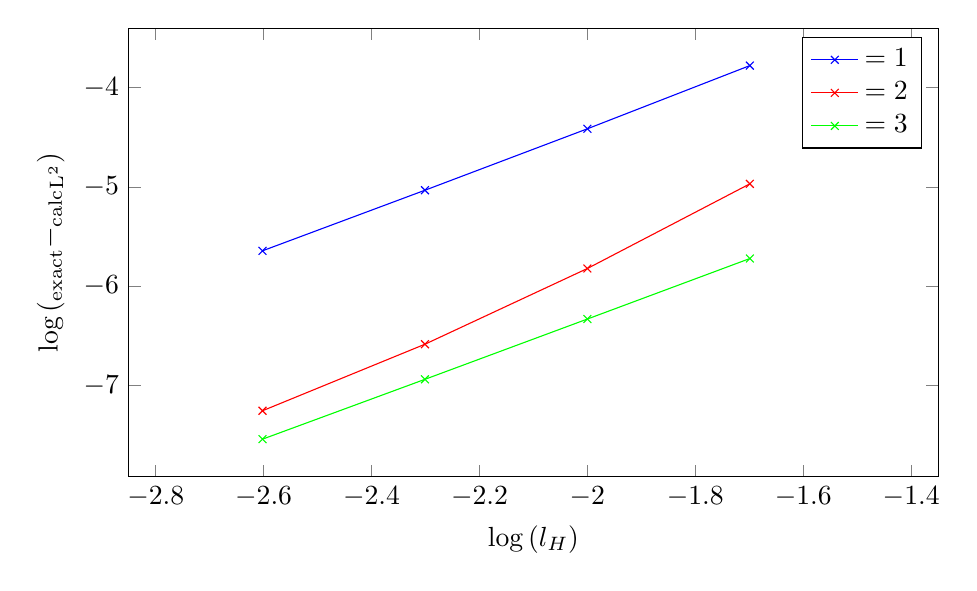
\begin{tikzpicture}[scale=1]
		\begin{axis}[
		%axis lines=middle,
		xlabel=$\log\left(l_H\right)$, %x label style={at={(axis cs:1.15,0)},anchor=north},
		ylabel=$\log\left(\Norm{\W_\mathrm{exact} - \W_\mathrm{calc}}_{\mathrm{L}^2}\right)$, %y label style={at={(axis cs:0,-0.05)},anchor=east},
		xmin=-2.85,xmax=-1.35,%ymin=-17,ymax=2,
		xtick={-2.8,-2.6,...,-1.4},%ytick={0,1},
		x post scale=1.5,
		%y post scale=2,
		%legend style={at={(axis cs:0.9,0.2)},anchor=south west}
		]
		
		\addplot+[color=blue,mark=x,] plot coordinates {
(-1.6989700043,	-3.7770339463)
(-2,	-4.4141390016)
(-2.3010299957,	-5.0335395886)
(-2.6020599913,	-5.6442593019)
		};
		\addlegendentry{$\Deg = 1$}
		
		\addplot+[color=red,mark=x,] plot coordinates {
(-1.6989700043,	-4.9691453617)
(-2,	-5.8224750429)
(-2.3010299957,	-6.5859011319)
(-2.6020599913,	-7.2567027309)
		};
		\addlegendentry{$\Deg = 2$}
		
		\addplot+[color=green,mark=x,] plot coordinates {
(-1.6989700043,	-5.7220494429)
(-2,	-6.3319795663)
(-2.3010299957,	-6.9397933789)
(-2.6020599913,	-7.5431907875)
		};
		\addlegendentry{$\Deg = 3$}
		
		\end{axis}
		\end{tikzpicture}
	\end{center}
\end{figure}

%ordre ref erreur
%1  5 1.67096e-04
%1 10 3.85355e-05
%1 20 9.25679e-06
%1 40 2.26851e-06
%
%2  5 1.07363e-05
%2 10 1.50496e-06
%2 20 2.59477e-07
%2 40 5.53729e-08
%
%3  5 1.89649e-06
%3 10 4.65608e-07
%3 20 1.14870e-07
%3 40 2.86292e-08

Nous mesurons aussi l'efficacité de la méthode en fonction de l'ordre
d'interpolation.
Pour cela nous simulons la même onde plane dans
le domaine délimité par le cube de côté $0.3$ m
et jusqu'au temps maximal $\Tmax = 1$ ns (figure~\ref{img:cv_sol_exacte}).
Ce domaine est maillé par des hexaèdres droits, tous identiques.
Nous utilisons la condition CFL \eqref{eq:cfl1}.
Nous mesurons les temps de calcul pour une subdivision en
$30$ mailles dans chaque direction à l'ordre $1$,
$15$ mailles dans chaque direction à l'ordre $2$ et
$10$ mailles dans chaque direction à l'ordre $3$.
Ces subdivisions génèrent des mailles dont la taille correspond
à l'application de la règle empirique du « $\lambda_{\min}$ sur $10$ ».
Nous sommes donc placés dans un cas discrétisé de manière équivalente
pour chaque ordre d'interpolation évalué.
Nous notons $T_\mathrm{s}(\Deg)$ le temps de simulation à l'ordre
d'interpolation $\Deg > 0$ pour	ce cas d'application.
\begin{definition}
	Dans les conditions décrites ci-avant, 
	l'\textbf{efficacité en fonction de l'ordre}
	d'interpolation spatiale $\Deg > 0$ du schéma couplé
	GD-RK$2$ est donnée par le rapport :
	\begin{align}
		E(\Deg) = \frac{T_\mathrm{s}(1)}{T_\mathrm{s}(\Deg)} .
	\end{align}
\end{definition}


\begin{figure}[!h]
	\begin{center}
		\caption{
			\label{img:cv_sol_exacte}
			Plan de coupe $(\x_1 O \x_3)$ en $\x_2 = 0.15$ m
			de la norme du champ électrique de la solution exacte de l'onde plane
			\eqref{eq:onde_plane} simulée, au temps final $\Tmax = 1$ ns.
		}
		
		\begin{tikzpicture}
		\begin{axis}[
		colormap/jet,
		colorbar,
		colorbar style={
			title={$\Norm{\E}$ (V/m)},
			%ylabel=Z-value,
			ytick={0,0.2,0.4,0.6,0.8,1},
			ymin=0,%ymax=2,
%			yticklabel style={
%				text width=2.5em,
%				align=right,
%				/pgf/number format/.cd,
%				fixed,
%				fixed zerofill
			},
		xlabel=$\x_1$, %x label style={at={(axis cs:1.15,0)},anchor=north},
		ylabel=$\x_3$, %y label style={at={(axis cs:0,-0.05)},anchor=east},	
		xtick={0,0.1,0.2,0.3},ytick={0,0.1,0.2,0.3},
		%tick label style={font=\tiny},
		view={0}{90}
		]
		%\addplot3 [surf, %domain = 0:0.3,
		%shader = interp,
		%domain y = 0:0.3, %samples = 350
		%] table[mark=none] {};
		\addplot3+[surf, shader = interp,
		domain = 0:0.3,
		domain y = 0:0.3,
		] table[mark=none] {plane_wave_exact_modE_xoz_t_1ns_y_15cm_mesh_cube30cm_ref_30.plt};
		\end{axis}
		\end{tikzpicture}
	\end{center}
\end{figure}

Les résultats d'efficacité sont présentés dans le tableau \ref{tab:order_time_struct}.
Nous pouvons constater qu'un ordre élevé est plus efficace et plus précis.
Cette différence d'efficacité est dûe au fait que le pas de temps est proportionnel
à la taille des mailles (plus grandes en ordre élevé)
et à la décroissance cubique de leur nombre avec la croissance de l'ordre.
Ces deux facteurs surcompensent l'augmentation de la complexité des calculs.


\begin{figure}[!h]
	\begin{center}
		\caption{
			\label{tab:order_time_struct}
			Efficacité du schéma couplé GD-RK$2$
			en fonction de l'ordre d'interpolation spatiale.
		}
		
		\begin{tabular}{|c|c|c|c|c|}
			\hline
			$\Deg$ & $\#\Mesh$ & $T_\mathrm{s}$ (en s) & $E(\Deg)$ & Erreur $\mathrm{L}^2$ \\ \hline\hline
			$1$ & $30^3$ & $11.6$ & $1$ & $2.35 \cdot 10^{-4}$ \\	\hline
			$2$ & $15^3$ & $2.06$ & $5.63$ & $5.45 \cdot 10^{-5}$ \\	\hline
			$3$ & $10^3$ & $1.30$ & $8.92$ & $3.79 \cdot 10^{-5}$ \\	\hline
		\end{tabular}
	\end{center}
\end{figure}

%cube de 30 cm
%t = 1 ns
%ordre	ref		time (s)	error
%1		30		13			2.35483e-04
%2		15		4.71		5.44504e-05
%3		10		3.34		3.78509e-05



\subsubsection{Maillage non structuré}
\label{sssect:cv_gd_rk2_non_struct}

Nous effectuons aussi les calculs de convergence du schéma couplé GD-RK$2$
sur maillage non structuré.
La convergence de la méthode GD appliquée
aux systèmes hyperboliques de lois de conservation
sur maillages non structurés a initialement
été démontrée par Szepessy \textit{et al.} \cite{SZEPESSY1}.


Nous maillons le même domaine délimité par le cube de côté $0.1$ m
en tétraèdres à l'aide du mailleur MeshGems commercialisé par Distene.
Ce domaine est maillé par des tétraèdres dont nous imposons la taille $l_T$ des arêtes
à $0.04$, $0.02$, $0.01$ et $0.005$ m, et qui sont ensuite découpés en hexaèdres
(figures \ref{img:tetra_hexa} et \ref{img:maillages_nstruct}) ayant respectivement une taille d'arête maximale,
notée $\max l_H$,
de $0.02$, $0.01$, $0.005$ et $0.0025$ m.
Ces tailles d'arête maximale correspondent à celles obtenues avec les subdivisions utilisées
en maillage structuré, à savoir des subdivisions respectives
en $5$, $10$, $20$ et $40$ mailles par côté.
Nous choisissons aussi le même temps maximal $\Tmax = 1$ ns.


\begin{figure}[!h]
	\begin{center}
		\caption{
			\label{img:maillages_nstruct}
			Faces $\x_2 O \x_3$ en $\x_1 = 0$
			des maillages non structurés
			utilisés pour les différentes tailles de maille.
		}
		
		\subfloat[$l_T = 0.04$ m.]{
			\label{img:maillages_nstruct_5}
			\begin{tikzpicture}[scale=50]
			\draw[thick] (0,0) rectangle (0.1,0.1);
			\input{cutplane_unstruct_5.plt}
			\end{tikzpicture}
		}
		\subfloat[$l_T = 0.02$ m.]{
			\label{img:maillages_nstruct_10}
			\begin{tikzpicture}[scale=50]
			\draw[thick] (0,0) rectangle (0.1,0.1);
			\input{cutplane_unstruct_10.plt}
			\end{tikzpicture}
		}
		\\
		\subfloat[$l_T = 0.01$ m.]{
			\label{img:maillages_nstruct_20}
			\begin{tikzpicture}[scale=50]
			\draw[thick] (0,0) rectangle (0.1,0.1);
			\input{cutplane_unstruct_20.plt}
			\end{tikzpicture}
		}
		\subfloat[$l_T = 0.005$ m.]{
			\label{img:maillages_nstruct_40}
			\begin{tikzpicture}[scale=50]
			\draw[thick] (0,0) rectangle (0.1,0.1);
			\input{cutplane_unstruct_40.plt}
			\end{tikzpicture}
		}
	\end{center}
\end{figure}


Le nombre de mailles contenues dans ces maillages non structurés
est généralement environ $4$ fois plus important que celui des maillages structurés correspondants.
De plus, la taille d'arête minimale est $4$ à $6$ fois inférieure
à la taille d'arête maximale, facteur impactant directement le pas de temps
et donc le nombre d'itérations de la méthode.
Nous pouvons donc estimer un temps de calcul en moyenne $23$ fois plus long
sur maillage non structuré issu de tétraèdres découpés,
par rapport à un maillage structuré équivalent
(tableau \ref{tab:comp_struct_nstruct}).


\begin{figure}[!h]
	\begin{center}
		\caption{
			\label{tab:comp_struct_nstruct}
			Comparaison des maillages structurés et non structurés
			utilisés dans le calcul de l'ordre de convergence du schéma couplé GD-RK$2$.
		}
		
		\subfloat[Comparaison en nombre de mailles.]{
			\label{tab:comp_struct_nstruct_nb_mailles}
		\begin{tabular}{|c|c|c|c|c|}
			\hline
			\multicolumn{2}{|c|}{\textbf{Structuré}} & \multicolumn{2}{c|}{\textbf{Non structuré}} & \multirow{2}{*}{\textbf{Facteur} $\bm{\#\Mesh}$} \\	\cline{1-4}
			Subdiv & $\#\Mesh$ & $l_T$ & $\#\Mesh$ & \\ \hline\hline
			$5$ & $125$ & $0.04$ & $508$ & $4.064$ \\	\hline
			$10$ & $1$k & $0.02$ & $4352$ & $4.352$ \\	\hline
			$20$ & $8$k & $0.01$ & $37408$ & $4.676$ \\	\hline
			$40$ & $64$k & $0.005$ & $304916$ & $4.764$ \\	\hline
		\end{tabular}
		}
		\\
		\subfloat[Comparaison en taille d'arêtes.]{
			\label{tab:comp_struct_nstruct_aretes}
		\begin{tabular}{|c|c|c|c|c|c|}
			\hline
			\multicolumn{2}{|c|}{\textbf{Structuré}} & \multicolumn{3}{c|}{\textbf{Non structuré}} & Inverse du \\	\cline{1-5}
			Subdiv & $l_H$ & $l_T$ & $\max l_H$ & $\min l_H$ & \textbf{Facteur} $\bm{(\min) l_H}$ \\ \hline\hline
			$5$ & $0.02$ & $0.04$ & $0.02$ & $0.004373$ & $4.574$ \\	\hline
			$10$ & $0.01$ & $0.02$ & $0.01$ & $0.002189$ & $4.568$ \\	\hline
			$20$ & $0.005$ & $0.01$ & $0.005$ & $0.000829$ & $6.031$ \\	\hline
			$40$ & $0.0025$ & $0.005$ & $0.0025$ & $0.000419$ & $5.967$ \\	\hline
		\end{tabular}
		}
	\end{center}
\end{figure}


Les résultats de convergence sont présentés dans la figure \ref{img:cv_non_struct}
pour les ordres d'interpolation $1$ à $3$.
Nous les présentons en fonction de la taille $l_T$ des arêtes des tétraèdres,
proportionnelle à la taille maximale $\max l_H$ des arêtes des hexaèdres, puisque ce paramètre
est l'indicateur de discrétisation du maillage.
Nous les présentons aussi en fonction de la taille minimale $\min l_H$ des arêtes des hexaèdres.

Ces résultats sont moins réguliers que sur maillage structuré (probablement)
car nous ne sommes pas dans le cas de raffinements d'un même maillage initial.
Nous constatons un ordre de convergence moyen d'environ $1.5$ à l'ordre spatial $\Deg = 1$
et supérieur à $2$ (mais toujours inférieur à $3$) pour les ordres $\Deg = 2$
et $\Deg = 3$.
\\


\begin{figure}[!h]
	\begin{center}
		\caption{
			\label{img:cv_non_struct}
			Convergence du schéma couplé GD-RK$2$
			appliqué aux équations de Maxwell en $3$ dimensions
			sur maillage non structuré.
		}
		
		\subfloat[Convergence en fonction de la taille $l_T$.]{
			\label{img:cv_non_struct_tetra}
		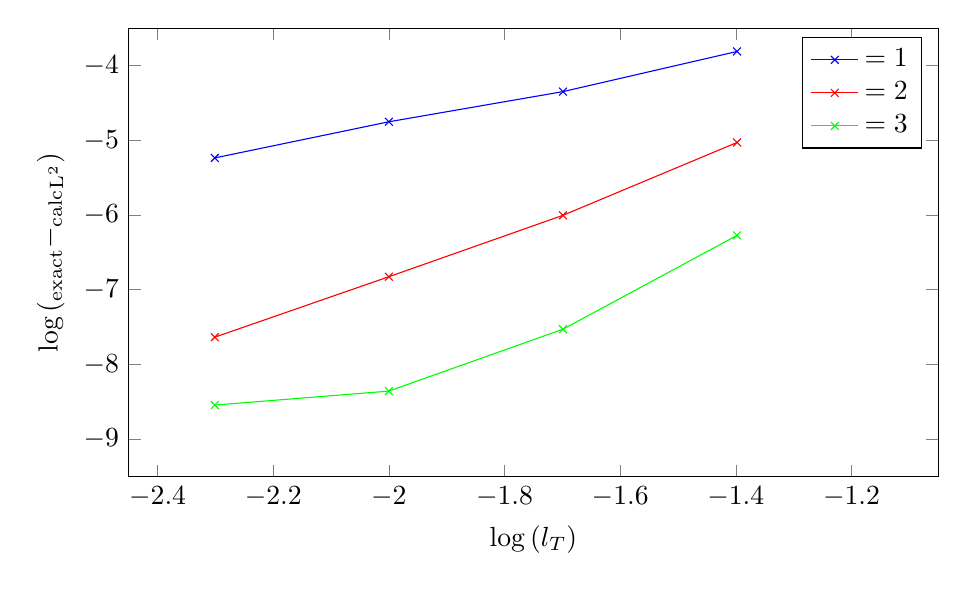
\begin{tikzpicture}[scale=1]
		\begin{axis}[
		%axis lines=middle,
		xlabel=$\log\left(l_T\right)$, %x label style={at={(axis cs:1.15,0)},anchor=north},
		ylabel=$\log\left(\Norm{\W_\mathrm{exact} - \W_\mathrm{calc}}_{\mathrm{L}^2}\right)$, %y label style={at={(axis cs:0,-0.05)},anchor=east},
		xmin=-2.45,xmax=-1.05,ymin=-9.5,ymax=-3.5,
		xtick={-2.4,-2.2,...,-1.0},ytick={-9,-8,...,-3},
		x post scale=1.5,
		%y post scale=2,
		%legend style={at={(axis cs:0.9,0.2)},anchor=south west}
		]
		
		\addplot+[color=blue,mark=x,] plot coordinates {
(-1.3979400087,	-3.810886032)
(-1.6989700043,	-4.3485097377)
(-2,	-4.7520439095)
(-2.3010299957,	-5.2358993711)
		};
		\addlegendentry{$\Deg = 1$}
		
		\addplot+[color=red,mark=x,] plot coordinates {
(-1.3979400087,	-5.0290787842)
(-1.6989700043,	-6.0040670429)
(-2,	-6.8257627874)
(-2.3010299957,	-7.6345700497)
		};
		\addlegendentry{$\Deg = 2$}
		
		\addplot+[color=green,mark=x,] plot coordinates {
(-1.3979400087,	-6.2732467178)
(-1.6989700043,	-7.5283460389)
(-2,	-8.3565157396)
(-2.3010299957,	-8.5435899323)
		};
		\addlegendentry{$\Deg = 3$}
		
% coeffs pentes vs taille tetra
% d=1
%1.7859472924
%1.3405115025
%1.607333052
%
% d=2
%3.2388408886
%2.729614179
%2.6867995681
%
% d=3
%4.1693496967
%2.751120196
%0.6214470164

		\end{axis}
		\end{tikzpicture}
		}
		\\
		\subfloat[Convergence en fonction de la taille $\min l_H$.]{
			\label{img:cv_non_struct_hexa}
		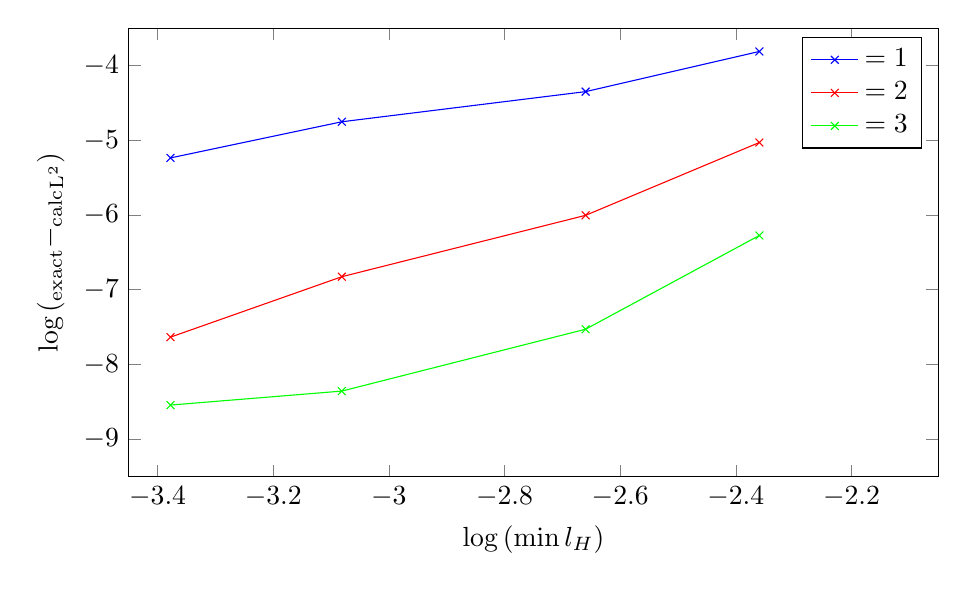
\begin{tikzpicture}[scale=1]
		\begin{axis}[
		%axis lines=middle,
		xlabel=$\log\left(\min l_H\right)$, %x label style={at={(axis cs:1.15,0)},anchor=north},
		ylabel=$\log\left(\Norm{\W_\mathrm{exact} - \W_\mathrm{calc}}_{\mathrm{L}^2}\right)$, %y label style={at={(axis cs:0,-0.05)},anchor=east},
		xmin=-3.45,xmax=-2.05,ymin=-9.5,ymax=-3.5,
		xtick={-3.4,-3.2,...,-2.0},ytick={-9,-8,...,-3},
		x post scale=1.5,
		%y post scale=2,
		%legend style={at={(axis cs:0.9,0.2)},anchor=south west}
		]
		
		\addplot+[color=blue,mark=x,] plot coordinates {
(-2.3592205227,	-3.810886032)
(-2.6597542384,	-4.3485097377)
(-3.0814454694,	-4.7520439095)
(-3.377785977,	-5.2358993711)
		};
		\addlegendentry{$\Deg = 1$}
		
		\addplot+[color=red,mark=x,] plot coordinates {
(-2.3592205227,	-5.0290787842)
(-2.6597542384,	-6.0040670429)
(-3.0814454694,	-6.8257627874)
(-3.377785977,	-7.6345700497)
		};
		\addlegendentry{$\Deg = 2$}
		
		\addplot+[color=green,mark=x,] plot coordinates {
(-2.3592205227,	-6.2732467178)
(-2.6597542384,	-7.5283460389)
(-3.0814454694,	-8.3565157396)
(-3.377785977,	-8.5435899323)
		};
		\addlegendentry{$\Deg = 3$}
		
% coeffs pentes vs taille hexa min
% d=1
%1.788896478
%0.9569422888
%1.6327685527
%
% d=2
%3.2441892789
%1.9485720452
%2.7293172605
%
% d=3
%4.1762346627
%1.9639244067
%0.6312812047

		\end{axis}
		\end{tikzpicture}
		}
	\end{center}
\end{figure}



\section{Tête humaine simplifiée}
\label{sect:tete_simplifiee}


Nous comparons le solveur \texttt{teta-clac} (Teta) au solveur Temsi-FD \cite{guiffaut2000contribution} (Temsi) qui implémente
la méthode des différences finies dans le domaine temporel (FDTD pour
« \textit{Finite Differences in Time Domain} ») et développé
à l'institut de recherche Xlim de Limoges.
Cette comparaison permet de confronter deux méthodes de calcul
implémentées par des équipes différentes et sur des architectures
distinctes car cet autre solveur utilise OpenMP (sur CPU).

Pour cela, nous comparons les résultats d'une simulation mettant en scène
une tête humaine simplifiée à proximité de laquelle nous avons placé une
antenne dipôle planaire de type ELPOSD
(pour « \textit{End-Loaded Planar Open-Sleeve Dipole} ») \cite{4020422}
conçue pour rayonner à une fréquence de $1$ GHz.
La particularité de cette antenne est que la source (la zone d'injection du signal) est un carré de côté
$1$ mm.
Cette forte contrainte géométrique diminue considérablement le pas de temps de simulation.
\\

\subsection{Description}
\label{ssect:tete_simplifiee_desc}


\subsubsection{Composition de la scène}

Cette simulation s'apparente au rayonnement d'une antenne de téléphone
mobile au cours d'une communication téléphonique.
L'antenne est placée à proximité de l'oreille de la tête simplifiée
et rayonne en direction du cerveau.

Dans notre cas d'étude, l'antenne est orientée dans le sens de la longueur
sur l'axe $(O\x_3)$, dans le sens de la largeur sur l'axe $(O\x_1)$
et rayonne dans la direction de l'axe $(O\x_2)$.
La tête simplifiée est placée de manière à ce que l'antenne rayonne
au niveau de son oreille droite, à $3.5$ cm de celle-ci.
Le centre de l'antenne se situe en $\Node{0}{0.113175}{0.12}$.
La tête simplifiée contient un cerveau simplifié délimité par un ellipsoïde.

Le domaine de calcul pour toutes les simulations de ce cas d'étude est 
un pavé de dimensions
$\ItvCC{-0.2}{0.2} \times \ItvCC{-0.2}{0.2} \times
\ItvCC{-0.1}{0.35}$ (en mètres), avant adjonction de
couches de PML (section \ref{ssect:PML}).


\begin{figure}[!h]
	\begin{center}
		\caption{
			\label{img:tete_elposd}
			Maillage en surfaces de l'antenne ELPOSD (en gris sombre)
			placée à proximité de la tête simplifiée.
			Scène vue depuis le côté positif de l'axe $(O\x_2)$.
			Une moitié de la surface délimitant la tête (en gris clair)
			est cachée pour laisser apparaître le cerveau (en rouge). 
		}
		
		\subfloat[Scène complète.]{
			\label{img:tete_elposd_all}
		\includegraphics[
			width=0.7\linewidth,
			trim={0 0 0 0},clip]{scene_brain}
		}
		\\
		\subfloat[Zoom sur la zone d'injection du signal (en blanc).]{
			\label{img:tete_elposd_zoom}
		\includegraphics[
			width=0.7\linewidth,
			trim={0 200 0 200},clip]{scene_brain_zoom}
		}
	\end{center}
\end{figure}



\subsubsection{Matériaux}

Nous appliquons le modèle PEC (section \ref{ssect:PEC}) sur
toute la surface de l'antenne, hormis la source.
La source nous permet d'injecter le signal dans la scène.

La tête contient des matériaux diélectriques dont les propriétés sont données dans le tableau \ref{tab:proprietes_mat_tete}. Nous utilisons les propriétés
de la matière grise dans le cerveau simplifié et celles
de la matière osseuse dans le reste de la tête simplifiée \cite{Gabriel1}.
Les propriétés électromagnétiques de ces matériaux sont
globalement constantes sur la bande de fréquences utilisée ($0.1$ à $10$ GHz).


\begin{figure}[!h]
	\begin{center}
		\caption{
			\label{tab:proprietes_mat_tete}
			Propriétés électromagnétiques des matériaux utilisés
			dans la scène de la tête simplifiée.
		}
		
		\begin{tabular}{|c|c|c|c|c|}
			\hline
			Matériau & $\EPrm_r$ & $\HPrm_r$ & $\ECnd$ (S/m) & $\HCnd$ \\ \hline\hline
			cerveau & $51.8$ & $1$ & $1.521$ & $0$ \\	\hline
			os & $11.41$ & $1$ & $0.43$ & $0$ \\	\hline
			vide & $1$ & $1$ & $0$ & $0$ \\	\hline
		\end{tabular}
	\end{center}
\end{figure}



\subsubsection{Signal source}

Dans le cas de la méthode FDTD, la zone d'injection
du signal, représentée par un carré de côté $1$ mm
situé au centre de l'antenne,
est remplacée par un fil d'excitation de rayon $0.125$ mm.
Ce fil implémente un modèle dérivé de celui de Holland \textit{et al.} \cite{4091427}
et qui peut s'appliquer aux fils obliques \cite{guiffaut:hal-00624720}.

Dans le cas de notre solveur GD, nous utilisons
le modèle de générateur de Thévenin (section \ref{ssect:the_venin})
sur la zone d'injection.
Pour les deux méthodes, nous appliquons le modèle
d'excitation avec une impédance réelle de $50$ Ohms.
\\

Le signal que nous utilisons pour les deux méthodes
est une impulsion gaussienne modulée
définie sur l'intervalle $\PbTps$ par :
%\todo{être plus précis: donner le champ EM complet E=... H=..}
\begin{align} \label{eq:onde_plane_mod}
	g : t \mapsto A \sin \left( 2 \pi \freq_0 \left( t - t_A \right) \right) \exp \left( -\left( \frac{t - t_A}{\tau} \right)^2 \right) ,
\end{align}
avec $A$ l'amplitude de l'onde,
$\freq_0$ la fréquence centrale du signal,
$\tau$ donnant l'intervalle de temps entre les deux points de demie-amplitude
(de largeur $2 \sqrt{\ln 2} \tau$) de l'impulsion gaussienne non modulée
et $t_A$ l'antécédent de la valeur d'amplitude maximale
(figure \ref{img:onde_plane_mod}).
Ce signal modulé est le produit d'une impulsion gaussienne
\eqref{eq:onde_plane} avec une sinusoïde.

Dans le cas de notre solveur GD, ce signal est injecté
sur toute la zone d'injection par le champ électrique incident
(section \ref{ssect:the_venin}) :
\begin{align}
	\E_I = \frac{g(t)}{50} \frac{\overrightarrow{O\x_3}}{0.001}
	= 20 g(t) \overrightarrow{O\x_3}
\end{align}
avec une impédance de surface de $50$ Ohm définie sur
cette même surface.
Le champ magnétique incident est nul.


\begin{figure}[!h]
	\begin{center}
		\caption{
			\label{img:onde_plane_mod}
			Signal adimensionné de la tension générée, utilisé
			au cours des simulations avec l'antenne ELPOSD.
		}
		
		\begin{tikzpicture}[scale=1]
		\begin{axis}[
		axis lines=middle,
		xlabel=$ct$, x label style={at={(axis cs:3.3,0)},anchor=north},
		ylabel=$0$, y label style={at={(axis cs:0,-0.1)},anchor=east},
		xmin=-0.3,xmax=3.3,ymin=-1.1,ymax=1.1,
		xtick={0,1,...,4},%ytick={0,0.5,1},
		x post scale=1.8,
		y post scale=1.5,
		%legend style={at={(axis cs:0.9,0.2)},anchor=south west}
		]
		
		\addplot+[
		mark=none,
		color=gray,
		dotted, thick,
		samples=200,
		domain=0:3
		]
		{exp(-((x-1.448)/0.5509)^2)};
		
		\addplot+[
		thick,
		mark=none,
		color=red,
		samples=500,
		domain=0:3
		] table {gauss_mod.plt};
		%{exp(-((x-1.448)/0.5509)^2)*sin(2*3.14159*10/3*(x-1.448))};
		
		\node[anchor=east] (a) at (axis cs:0.9893456647,0.5){};
		\node[anchor=west] (b) at (axis cs:1.9066543353,0.5){};
		\draw[arrows={latex-latex}](a)--node[midway,below]{$2 \sqrt{\ln 2} \tau$}(b);
		
		\node[anchor=east] (c) at (axis cs:0,1){};
		\node[anchor=west] (d) at (axis cs:1.448,1){};
		\draw[dotted](c)--(d);
		
		\node[anchor=east] (e) at (axis cs:0,0.5){};
		\node[anchor=west] (f) at (axis cs:0.9893456647,0.5){};
		\draw[dotted](e)--(f);
		
		\node[anchor=north] (g) at (axis cs:1.448,0){};
		\node[anchor=south] (h) at (axis cs:1.448,1){};
		\draw[dotted](g)--(h);
		
		\node[anchor=north west] at (axis cs:1.448,0){$t_A$};
		\node[anchor=north west] at (axis cs:0,1){$A$};
		
		\end{axis}
		\end{tikzpicture}
	\end{center}
\end{figure}


Les paramètres $\tau$ et $t_A$ sont donnés par les relations suivantes :
\begin{subequations}
	\begin{align}
	\tau &= 2 \frac{\sqrt{- \ln (a_A)}}{\pi \Delta_\freq} ,
	\\
	t_A &= \tau \sqrt{- \ln (a_0)} ,
	\end{align}
\end{subequations}
où $a_0$ représente l'atténuation au temps initial ($t=0$),
$a_A$ représente l'atténuation au temps d'amplitude maximale $t_A$
et $\Delta_\freq$ représente la largeur de la bande de 
fréquences du signal considéré, centrée en $\freq_0$.

Pour notre cas d'application nous choisissons :
\begin{itemize}
	\item $A = 1$ ;
	\item $\freq_0 = 1$ GHz ;
	\item $\Delta_\freq = 0.6$ GHz ;
	\item $a_0 = 0.001$ (ou $0.1$ \%).
	\item $a_A = 0.05$ (ou $5$ \%) ;
\end{itemize}
Avec ces valeurs, dans le cas adimensionné,
nous avons $\tau \approx 0.5509$ et $t_A \approx 1.448$,
ce qui nous donne une durée de signal d'environ $10$ ns.


\subsubsection{Maillage}


La fréquence maximale considérée est de $\freq_{\max} =
\freq_0 + \Delta_\freq / 2 = 1.3$ GHz.
Le tableau \ref{tab:dx_mat_tete} présente la distance maximale
entre deux points d'interpolation 
selon la règle empirique du « $\lambda_{\min}$ sur $10$ »
en fonction des propriétés électromagnétiques des matériaux
à la fréquence $\freq_{\max} = 1.3$ GHz
(tableau~\ref{tab:proprietes_mat_tete}).


\begin{figure}[!h]
	\begin{center}
		\caption{
			\label{tab:dx_mat_tete}
			Distances maximales
			entre deux points d'interpolation
			en fonction des matériaux
			à la fréquence $1.3$ GHz.
		}
		
		\begin{tabular}{|c|c|c|}
			\hline
			Matériau & $\dx$ (mm) & $l_T$, $\Deg = 2$ (mm) \\ \hline\hline
			cerveau & $3.2$ & $12.8$ \\	\hline
			os & $6.8$ & $27.2$ \\	\hline
			vide & $23$ & $92$ \\	\hline
		\end{tabular}
	\end{center}
\end{figure}


Pour obtenir la taille d'arête maximale d'un hexaèdre à partir
de ces valeurs,
nous devons les multiplier par l'ordre d'interpolation spatiale choisi.
Dans le cas d'un maillage en tétraèdres, nous devons considérer
le double des arêtes des hexaèdres, afin d'appliquer le découpage
présenté en figure \ref{img:tetra_hexa}.

Pour une simulation à l'ordre d'interpolation spatiale $\Deg=2$,
nous maillons donc la scène avec les longueurs d'arête de tétraèdre $l_T$
données dans la dernière colonne du tableau \ref{tab:dx_mat_tete}.
Pour cela, nous commençons par mailler les surfaces avec la plus
petite taille d'arête à appliquer sur les volumes voisins
($12.8$ mm pour la peau du cerveau et $27.2$ pour la peau de la tête),
puis nous maillons les volumes.

L'antenne ELPOSD a préalablement été maillée avec une taille d'arête
maximale de $10$ mm afin d'assurer un rayonnement de bonne qualité.
Les champs électromagnétiques obtenus avec cette finesse de maillage correspondent
à ceux obtenus sur une version maillée à une taille d'arête maximale de $5$ mm
(figure \ref{img:rayonnement_elposd}) ainsi que ceux obtenus dans le cas de la méthode FDTD.
Dans le cas de l'antenne maillée à une taille d'arête maximale de $15$ mm,
nous observons une dégradation des résultats en fin de signal
(figure~\ref{img:rayonnement_elposd_zoom}).

\begin{figure}[!h]
	\begin{center}
		\caption{
			\label{img:rayonnement_elposd}
			Composante $\x_3$ du champ $\E$ au point
			$\Node{0}{0.095675}{0.12}$ (à mi-chemin de la distance
			antenne-oreille) dans une configuration « antenne seule ».
			Comparaison à la méthode FDTD pour différents raffinements de l'antenne
			dans le cas du schéma couplé GD-RK$2$.
		}
		
		\subfloat[Signal complet.]{
			\label{img:rayonnement_elposd_full}
		\begin{tikzpicture}[scale=1]
		\begin{axis}[
		axis lines=middle,
		xlabel=$t$ (ns),% x label style={at={(axis cs:0.5,0)},anchor=north},
		ylabel=$\E$ (V/m),% y label style={at={(axis cs:0,-0.05)},anchor=east},
		xmin=0,xmax=11,%ymin=-0.1,ymax=1.1,
		xtick={0,1,...,10},ytick={-6,-4,...,6},
		x post scale=1.8,
		y post scale=1.2,
		%legend style={at={(axis cs:0.9,0.2)},anchor=south west}
		]
		
		\addplot+[
		smooth,
		%thick,
		mark=none,
		color=red,
		] table
		{elposd/temsi_ez_p1.plt};
		\addlegendentry{Temsi @ $1$ mm}
		
		\addplot+[
		%thick,
		mark=none,
		color=blue,
		densely dashed,
		] table
		{elposd/teta_ez_p1_5mm.plt};
		\addlegendentry{Teta @ $5$ mm}
		
		\addplot+[
		%thick,
		mark=none,
		color=green,
		densely dotted,
		] table
		{elposd/teta_ez_p1_10mm.plt};
		\addlegendentry{Teta @ $10$ mm}
		
		\addplot+[
		%thick,
		mark=none,
		color=orange,
		densely dashdotted,
		] table
		{elposd/teta_ez_p1_15mm.plt};
		\addlegendentry{Teta @ $15$ mm}

		\end{axis}
		\end{tikzpicture}
		}
		\\
		\subfloat[Agrandissement de la zone d'intérêt.]{
			\label{img:rayonnement_elposd_zoom}
		\begin{tikzpicture}[scale=1]
		\begin{axis}[
		axis lines=middle,
		xlabel=$t$ (ns),% x label style={at={(axis cs:0.5,0)},anchor=north},
		ylabel=$\E$ (V/m),% y label style={at={(axis cs:0,-0.05)},anchor=east},
		xmin=7,xmax=10,ymin=-1.6,ymax=2.2,
		xtick={7,7.5,...,9.5},ytick={-1,-0.5,...,2},
		x post scale=1.8,
		y post scale=1.2,
		%legend style={at={(axis cs:0.9,0.2)},anchor=south west}
		]
		
		\addplot+[
		smooth,
		%thick,
		mark=none,
		color=red,
		] table
		{elposd/temsi_ez_p1.plt};
		\addlegendentry{Temsi @ $1$ mm}
		
		\addplot+[
		%thick,
		mark=none,
		color=blue,
		densely dashed,
		] table
		{elposd/teta_ez_p1_5mm.plt};
		\addlegendentry{Teta @ $5$ mm}
		
		\addplot+[
		%thick,
		mark=none,
		color=green,
		densely dotted,
		] table
		{elposd/teta_ez_p1_10mm.plt};
		\addlegendentry{Teta @ $10$ mm}
		
		\addplot+[
		%thick,
		mark=none,
		color=orange,
		densely dashdotted,
		] table
		{elposd/teta_ez_p1_15mm.plt};
		\addlegendentry{Teta @ $15$ mm}
		
		
		\end{axis}
		\end{tikzpicture}
		}
	\end{center}
\end{figure}

Après cette phase de maillage, nous obtenons un ensemble de $19413$ tétraèdres.
En résultent $77652$ hexaèdres quelconques après le découpage des tétraèdres,
auxquels s'ajoutent $4570$ hexaèdres droits en bordure de domaine pour
l'application du modèle PML.
Les surfaces présentées dans la figure \ref{img:tete_elposd}
sont issues de ce maillage.
\\

Dans le cas de la méthode FDTD, la zone d'injection
du signal, représentée par un carré de côté $1$ mm
situé au centre de l'antenne,
impose le pas de discrétisation.
Cette méthode de calcul nécessite de discrétiser la scène en mailles
hexaédriques sous la forme d'une grille structurée.
Le maillage résultant est composé d'environ $77.5$ millions de mailles
($417 \times 428 \times 434$).
Le modèle PML ajoute environ $12$ millions de mailles en bordure
de domaine.
Nous avons donc une grille structurée composée d'un peu moins de $90$ millions
de mailles de côté $1$ mm.
Soit un nombre de mailles $1087$ fois plus important que pour la méthode GD.
\\


\subsection{Comparaison à la méthode FDTD}
\label{ssect:tete_simplifiee_comp}

\subsubsection{Mémoire}
\label{sssect:tete_simplifiee_comp_mem}

Du point de vue de la mémoire, la simulation GD occupe $380$ Mo sur le GPU
(avec environ $100$ Mo supplémentaires pour l'allocation des instances OpenCL)
contre environ $9$ Go en RAM dans le cas de la simulation FDTD, soit
$23$ fois moins de mémoire utile pour la méthode GD.

Cette différence d'occupation en mémoire est principalement liée à la quantité de mailles
et aux degrés de liberté par maille. Dans le cas de la méthode GD,
la nature non structurée du maillage nécessite aussi de stocker une grande
quantité de coordonnées et d'informations de connectivité entre les mailles.


\subsubsection{Performances}
\label{sssect:tete_simplifiee_comp_perfs}

En temps de calcul, la simulation FDTD sur grille structurée a nécessité $4.85$ heures
pour simuler $20$ ns de temps physique sur $22$ cœurs (logiques) d'un processeur
Intel Dual Xeon E5645 ($2 \times 6$ cœurs physiques hyperthreadés) cadencé à $2.40$ GHz.
Le temps de calcul sur $46$ cœurs (logiques) du plus récent processeur Intel Dual Xeon E5-2650 v4
($2 \times 12$ cœurs physiques hyperthreadés) cadencé à $2.20$ GHz est de $2.24$ heures.
Le coefficient CFL imposé par la largeur du fil d'excitation est de $0.92$
et le pas de temps de la simulation est calculé à $1.772 \cdot 10^{-12}$ s
par la condition CFL classique utilisée avec la méthode FDTD.
\\


Dans le cas de la méthode GD sur maillage non structuré à l'ordre spatial $\Deg=2$,
la simulation a nécessité $1.88$ heures de
calcul sur un GPU NVidia GeForce GTX 1070 cadencé à $1.721$ GHz
et $1.19$ heures de
calcul sur un GPU NVidia GeForce GTX 1080 Ti cadencé à $1.582$ GHz.

L'application du diagnostic de la puissance itérée (section \ref{ssect:puissance itérée})
nous a permis de constater que dans le cas ce cette simulation, la condition
CFL de stabilité \eqref{eq:cfl1} sous-évalue le pas de temps de stabilité.
Nous avons fixé le coefficient CFL à $3.1$ et utilisé la formule \eqref{eq:cfl1}
pour le calcul du pas de temps de la simulation.
Le pas de temps ainsi obtenu est de $6.641 \cdot 10^{-14}$ s,
soit $27$ fois plus petit que celui utilisé dans le cas de la méthode FDTD.
\\

Les performances des deux solveurs peuvent donc être considérées du même ordre de grandeur
sur ce cas d'application.
Bien que la méthode GD soit présentée comme étant plus rapide que la méthode
FDTD, le temps de restitution est fonction du support de calcul utilisé.
Les temps de calculs obtenus sont résumés dans le tableau \ref{tab:tete_elposd_times}.

La méthode GD est très bien adaptée dans ce cas d'application compte tenu du
facteur d'échelle (proche de $100$) entre la plus petite et la plus grande maille du maillage. La méthode FDTD quant à elle, est directement affectée par la plus petite
maille qui impose le pas spatial de la grille structurée.


\begin{figure}[!h]
	\begin{center}
		\caption{
			\label{tab:tete_elposd_times}
			Temps de calcul des méthodes GD et FDTD en fonction
			du support d'exécution dans le cas de la simulation de
			l'antenne ELPOSD placée à proximité de la tête humaine simplifiée.
		}
		
		\begin{tabular}{|c|c|c|c|}
			\hline
			Solveur & Support d'exécution & CFL & Temps (h) \\ \hline\hline
			\multirow{2}{*}{Temsi} & Dual Xeon E5645, 22 threads & $0.92$ & $4.85$ \\	\cline{2-4}
			& Dual Xeon E5-2650 v4, 46 threads & $0.92$ & $\bm{2.24}$ \\	\hline
			\multirow{2}{*}{Teta} & GeForce GTX 1070 & $3.1$ & $1.88$ \\	\cline{2-4}
			& GeForce GTX 1080 Ti & $3.1$ & $\bm{1.19}$ \\	\hline
		\end{tabular}
	\end{center}
\end{figure}


\subsubsection{Résultats}
\label{sssect:tete_simplifiee_comp_res}

La figure \ref{img:tete_elposd_cutplane} présente un plan de coupe
des résultats de la simulation par la méthode GD.


\begin{figure}[!h]
	\begin{center}
		\caption{
			\label{img:tete_elposd_cutplane}
			Plan de coupe $(\x_1 O \x_2)$ en $\x_3 = 0.12$ m
			du logarithme (10dB) de la norme du champ électrique de la solution
			calculée dans le cas de la simulation de l'antenne ELPOSD
			placée à proximité de la tête humaine simplifiée
			au temps $t=3$ ns.
			Discrétisation à $5$ mm.
			La zone rouge correspond au centre de l'antenne, la zone
			bleue foncée correspond à la tête simplifiée.
		}
		
		\begin{tikzpicture}
		\begin{axis}[
		colormap/jet,
		colorbar,
		colorbar style={
			title={$\Norm{\E}$ (dBV/m)},
			%ylabel=Z-value,
			%ytick={0,0.2,0.4,0.6,0.8,1},
			%ymin=0,%ymax=2,
			%			yticklabel style={
			%				text width=2.5em,
			%				align=right,
			%				/pgf/number format/.cd,
			%				fixed,
			%				fixed zerofill
		},
		xlabel=$\x_1$, %x label style={at={(axis cs:1.15,0)},anchor=north},
		ylabel=$\x_2$, %y label style={at={(axis cs:0,-0.05)},anchor=east},	
		xtick={-0.2,-0.1,0,0.1,0.2},
		ytick={-0.2,-0.1,0,0.1,0.2},
		%tick label style={font=\tiny},
		view={0}{90},
		x post scale=1.4,
		y post scale=1.6,
		]

		\addplot3+[surf,%shader=interp,
		%patch type=rectangle,
		domain = -0.202285:0.212715,
		domain y = -0.205175:0.219825,
		mesh/rows=84,
		mesh/cols=86,
		] table[mark=none] {tete_elposd/teta_tete_elposd_xoy_t_3ns.plt};

%		\addplot3+[surf,%shader=interp,
%		%patch type=rectangle,
%		domain = -0.202285:0.213715,		
%		domain y = -0.205175:0.221825,		
%		mesh/rows=417,
%		mesh/cols=428,
%		] table[mark=none] {tete_elposd/teta_tete_elposd_xoy_t_3ns_1mm.plt};
		\end{axis}
		\end{tikzpicture}
	\end{center}
\end{figure}


Ces résultats sont très proches de ceux obtenus avec la méthode FDTD.
Afin de faciliter la comparaison, 
nous présentons aussi la valeur de la composante $\x_3$ du champ électrique
mesuré en différents points d'observation (figure \ref{img:tete_elposd_curves}) :
\begin{itemize}
	\item en $O_1 = \Node{0}{0.095675}{0.12}$, à mi-chemin entre l'antenne et la tête ;
	\item en $O_2 = \Node{0}{0}{0.12}$, à l'intérieur du cerveau, à hauteur de la zone
	source de l'antenne ;
	\item en $O_3 = \Node{0}{-0.113175}{0.12}$, le symétrique de la zone
	source de l'antenne par rapport au point $O_2$.
\end{itemize}


\begin{figure}[!h]
	\centering
		\caption{
			\label{img:tete_elposd_curves}
			Valeur de la composante $\x_3$ du champ électrique
			mesuré en différents points d'observation dans le cas de la simulation de
			l'antenne ELPOSD placée à proximité de la tête humaine simplifiée.
			Comparaison de la méthode FDTD au schéma couplé GD-RK$2$.
		}

		\subfloat[Au point $O_1$.]{
			\centering
			\label{img:tete_elposd_curves_O1}
			\begin{tikzpicture}[scale=0.8]
			\begin{axis}[
			axis lines=middle,
			xlabel=$t$ (ns), x label style={at={(axis cs:11.5,0)},anchor=south},
			ylabel=$\E$ (V/m), y label style={at={(axis cs:0,6)},anchor=west},
			xmin=0,xmax=13,%ymin=-0.1,ymax=1.1,
			xtick={0,2,...,12},%ytick={0,0.5,1},
			%x post scale=1.8,
			%y post scale=1.2,
			%legend style={at={(axis cs:0.9,0.2)},anchor=south west}
			]
			
			\addplot+[
			%thick,
			mark=none,
			color=red,
			] table
			[y expr=-\thisrowno{1}]
			{tete_elposd/temsi_ez_O1.plt};
			%\addlegendentry{Temsi}
			
			\addplot+[
			%thick,
			mark=none,
			color=blue,
			densely dashed,
			] table
			{tete_elposd/teta_ez_O1.plt};
			%\addlegendentry{Teta}
			
			\end{axis}
			\end{tikzpicture}
		}
		\hfill
		\subfloat[Au point $O_2$.]{
			\centering
			\label{img:tete_elposd_curves_O2}
			\begin{tikzpicture}[scale=0.8]
			\begin{axis}[
			axis lines=middle,
			xlabel=$t$ (ns), x label style={at={(axis cs:11.5,0)},anchor=south},
			ylabel=$\E$ (V/m), y label style={at={(axis cs:0,0.175)},anchor=west},
			xmin=0,xmax=13,%ymin=-0.1,ymax=1.1,
			xtick={0,2,...,12},%ytick={0,0.5,1},
			%x post scale=1.8,
			%y post scale=1.2,
			%legend style={at={(axis cs:0.9,0.2)},anchor=south west}
			]
			
			\addplot+[
			%thick,
			mark=none,
			color=red,
			] table
			[y expr=-\thisrowno{1}]
			{tete_elposd/temsi_ez_O2.plt};
			\addlegendentry{Temsi}
			
			\addplot+[
			%thick,
			mark=none,
			color=blue,
			densely dashed,
			] table
			{tete_elposd/teta_ez_O2.plt};
			\addlegendentry{Teta}
			
			\end{axis}
			\end{tikzpicture}

		}	
		\\
		\subfloat[Au point $O_3$.]{
			\centering
			\label{img:tete_elposd_curves_O3}
			\begin{tikzpicture}[scale=0.8]
			\begin{axis}[
			axis lines=middle,
			xlabel=$t$ (ns), x label style={at={(axis cs:11.5,0)},anchor=south},
			ylabel=$\E$ (mV/m), y label style={at={(axis cs:0,70)},anchor=west},
			xmin=0,xmax=13,%ymin=-0.1,ymax=1.1,
			xtick={0,2,...,12},%ytick={0,0.5,1},
			%x post scale=1.8,
			%y post scale=1.2,
			%legend style={at={(axis cs:0.9,0.2)},anchor=south west}
			]
			
			\addplot+[
			%thick,
			mark=none,
			color=red,
			] table
			[y expr=-\thisrowno{1}*1000]
			{tete_elposd/temsi_ez_O3.plt};
			%\addlegendentry{Temsi}
			
			\addplot+[
			%thick,
			mark=none,
			color=blue,
			densely dashed,
			] table
			[y expr=\thisrowno{1}*1000]
			{tete_elposd/teta_ez_O3.plt};
			%\addlegendentry{Teta}
			
			\end{axis}
			\end{tikzpicture}
		}	
		\hfill
		\subfloat[Position des points.]{
			\centering
			\label{img:tete_elposd_curves_pos}
			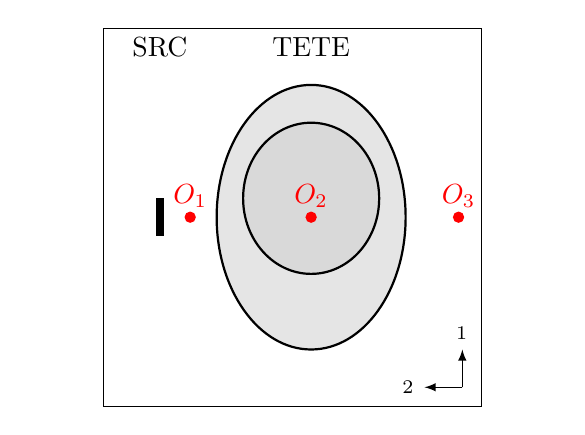
\begin{tikzpicture}[scale=4.8]
			\fill[white] (-0.2,0) rectangle (1.2,1);
			\draw (0,0) rectangle (1,1);
			\fill (0.14,0.45) rectangle (0.16,0.55);
			\draw[thick,fill=gray!20] (0.55,0.5) ellipse (0.25 and 0.35);
			\draw[thick,fill=gray!30] (0.55,0.55) ellipse (0.18 and 0.2);
			\draw (0.15,1) node[below] {SRC};
			\draw (0.55,1) node[below] {TETE};
			\draw[arrows={-latex}] (0.95,0.05) -- (0.95,0.15) node[above] {$\x_1$};
			\draw[arrows={-latex}] (0.95,0.05) -- (0.85,0.05) node[left] {$\x_2$};
			\fill[red] (0.23,0.5) circle (0.015) node[above,red]{$O_1$};
			\fill[red] (0.55,0.5) circle (0.015) node[above,red]{$O_2$};
			\fill[red] (0.94,0.5) circle (0.015) node[above,red]{$O_3$};
			\end{tikzpicture}
		}	
\end{figure}

Nous constatons que les deux solveurs produisent sensiblement les mêmes
résultats. Un léger décalage peut être constaté dans le cas des
mesures effectuées à l'intérieur du cerveau et de l'autre côté de la tête
par rapport à l'antenne.
Entre la tête et l'antenne, les résultats sont identiques.

Nous pouvons aussi remarquer que l'onde électromagnétique atteint le côté opposé
de la tête avant le centre du cerveau. Ces résultats sont dûs à la forte permittivité
des matériaux de la tête qui diminuent la vitesse de propagation des ondes.
Cette propriété des matériaux génère le phénomène d'« enroulement »
des ondes constaté au niveau de la zone du cerveau sur la figure \ref{img:tete_elposd_cutplane}.
\\

Nous avons évoqué d'autres axes d'optimisation dans les chapitres précédents.
Du point du vue de la discrétisation spatiale, nous pouvons réduire la masse
de calculs en appliquant l'ordre spatial adaptatif.
Nous avons aussi décrit une méthode d'intégration avec application d'un pas de temps
local par maille.
Les résultats et perfomances obtenues avec ces deux méthodes sont
présentés dans les sections suivantes.



\subsection{Application de l'ordre spatial adaptatif}
\label{ssect:tete_simplifiee_adaptatif}

Le découpage des tétraèdres génère des hexaèdres dont la taille $\min l_H$
de la plus petite arête peut être jusqu'à $6$ fois inférieure à la taille
donnée par l'application de la règle du « $\lambda_{\min}$ sur $10$ »
(tableau \ref{tab:comp_struct_nstruct_aretes}).
Nous pouvons donc appliquer un ordre
d'interpolation spatiale inférieur sur ces mailles (section~\ref{sect:ordre_adaptatif})
tout en conservant
un raffinement suffisant du point de vue de l'évaluation du pas de temps
de simulation (application du critère CFL \eqref{eq:cfl1} sur la plus petite
arête de chaque maille devant respecter la règle du « $\lambda_{\min}$ sur $10$ »).

Rappelons que nous imposons un ordre spatial minimal à $\Deg=1$. Ainsi,
la plupart des mailles de notre simulation passent à cet ordre d'interpolation.
Seuls les hexaèdres droits générés en bordure de domaine pour l'application du modèle PML
ont une taille suffisante pour conserver un ordre spatial $2$.
Du point de vue de la discrétisation spatiale (théorème de Shannon
sur l'échantillonnage des signaux),
le passage de l'ordre $2$ à l'ordre $1$ implique une discrétisation
proche de « $\lambda_{\min}$ sur $5$ » à proximité des arêtes les plus longues.
Cet échantillonnage est suffisant pour représenter fidèlement les ondes.

Le maillage ainsi que les paramètres de simulation (hormis les ordres d'interpolation)
sont identiques à ceux présentés dans la section \ref{ssect:tete_simplifiee_desc}.
Nous obtenons donc une simulation composée de $77652$ hexaèdres quelconques
spatialement interpolés à l'ordre $1$ et $4570$ hexaèdres droits en bordure de domaine
pour l'application du modèle PML interpolés à l'ordre $2$.


\subsubsection{Performances}

Cette simulation a duré $0.31$ heures sur NVidia GeForce GTX 1080 Ti
avec l'application du coefficient CFL $4.5$ déterminé par la méthode de la puissance
itérée pour l'ordre d'interpolation spatiale $\Deg=1$.
Les mailles du modèle PML sont suffisamment grandes pour être stables
avec ce coefficient CFL.
Le pas de temps de la simulation est de $1.446 \cdot 10^{-13}$ s.

Une accélération d'un facteur $3.8$
par rapport à la même simulation interpolant spatialement à l'ordre
$\Deg=2$ sur toutes les mailles est donc constaté.


\subsubsection{Résultats}

Les résultats sont proches de ceux obtenus avec une interpolation
homogène à l'ordre $2$.
Nous constatons cependant une légère
perte dans l'amplitude du signal ($-5$ \%), dès son injection
via le modèle de générateur de Thévenin (section \ref{ssect:the_venin}).

L'amplitude du signal au niveau du point de mesure $O_3$,
situé de l'autre côté de la tête, est plus faible que celle
mesurée pour l'ordre $2$. Ceci témoigne du fait que l'interpolation
spatiale à l'ordre $1$ est plus dissipative qu'une interpolation à l'ordre $2$.
En effet, nous passons de fonctions de base quadratiques à des fonctions linéaires,
l'approximation est donc moins précise.
L'amplitude du signal au niveau du point de mesure $O_2$,
situé dans le cerveau, est quant à elle plus importante 
que celle mesurée pour l'ordre $2$.

Toutefois, mises à part les différences d'amplitude, la forme du signal est fidèle
au signal mesuré pour une interpolation à l'ordre $2$.
La perte de précision est naturellement induite par l'utilisation d'un ordre
d'interpolation inférieur, et spécialement dans le cas de l'ordre $1$
qui linéarise (par morceaux) l'approximation de la solution.
Il est donc préférable d'appliquer l'ordre adaptatif dans le cas
d'une interpolation initiale d'ordre plus élevé.
\\

\begin{figure}[!h]
	\centering
	\caption{
		\label{img:tete_elposd_adapt_curves}
		Valeur de la composante $\x_3$ du champ électrique
		mesuré en différents points d'observation dans le cas de la simulation de
		l'antenne ELPOSD placée à proximité de la tête humaine simplifiée.
		Comparaison du schéma couplé GD-RK$2$ pour $\Deg=2$ au même schéma
		avec application de l'ordre d'interpolation spatiale adaptatif ($d\le2$).
	}
	
	\subfloat[Au point $O_1$.]{
		\centering
		\label{img:tete_elposd_adapt_curves_O1}
		\begin{tikzpicture}[scale=0.8]
		\begin{axis}[
		axis lines=middle,
		xlabel=$t$ (ns), x label style={at={(axis cs:11.5,0)},anchor=south},
		ylabel=$\E$ (V/m), y label style={at={(axis cs:0,6)},anchor=west},
		xmin=0,xmax=13,%ymin=-0.1,ymax=1.1,
		xtick={0,2,...,12},%ytick={0,0.5,1},
		%x post scale=1.8,
		%y post scale=1.2,
		%legend style={at={(axis cs:0.9,0.2)},anchor=south west}
		]
		
		\addplot+[
		%thick,
		mark=none,
		color=red,
		] table
		{tete_elposd/teta_ez_O1.plt};
		%\addlegendentry{Temsi}
		
		\addplot+[
		%thick,
		mark=none,
		color=blue,
		densely dashed,
		] table
		{tete_elposd/teta_ez_O1_adapt.plt};
		%\addlegendentry{Teta}
		
		\end{axis}
		\end{tikzpicture}
	}
	\hfill
	\subfloat[Au point $O_2$.]{
		\centering
		\label{img:tete_elposd_adapt_curves_O2}
		\begin{tikzpicture}[scale=0.8]
		\begin{axis}[
		axis lines=middle,
		xlabel=$t$ (ns), x label style={at={(axis cs:11.5,0)},anchor=south},
		ylabel=$\E$ (V/m), y label style={at={(axis cs:0,0.175)},anchor=west},
		xmin=0,xmax=13,%ymin=-0.1,ymax=1.1,
		xtick={0,2,...,12},%ytick={0,0.5,1},
		%x post scale=1.8,
		%y post scale=1.2,
		%legend style={at={(axis cs:0.9,0.2)},anchor=south west}
		]
		
		\addplot+[
		%thick,
		mark=none,
		color=red,
		] table
		{tete_elposd/teta_ez_O2.plt};
		\addlegendentry{$\Deg=2$}
		
		\addplot+[
		%thick,
		mark=none,
		color=blue,
		densely dashed,
		] table
		{tete_elposd/teta_ez_O2_adapt.plt};
		\addlegendentry{$d\le2$}
		
		\end{axis}
		\end{tikzpicture}
		
	}	
	\\
	\subfloat[Au point $O_3$.]{
		\centering
		\label{img:tete_elposd_adapt_curves_O3}
		\begin{tikzpicture}[scale=0.8]
		\begin{axis}[
		axis lines=middle,
		xlabel=$t$ (ns), x label style={at={(axis cs:11.5,0)},anchor=south},
		ylabel=$\E$ (mV/m), y label style={at={(axis cs:0,70)},anchor=west},
		xmin=0,xmax=13,%ymin=-0.1,ymax=1.1,
		xtick={0,2,...,12},%ytick={0,0.5,1},
		%x post scale=1.8,
		%y post scale=1.2,
		%legend style={at={(axis cs:0.9,0.2)},anchor=south west}
		]
		
		\addplot+[
		%thick,
		mark=none,
		color=red,
		] table
		[y expr=\thisrowno{1}*1000]
		{tete_elposd/teta_ez_O3.plt};
		
		\addplot+[
		%thick,
		mark=none,
		color=blue,
		densely dashed,
		] table
		[y expr=\thisrowno{1}*1000]
		{tete_elposd/teta_ez_O3_adapt.plt};
		
		\end{axis}
		\end{tikzpicture}
	}	
	\hfill
	\subfloat[Position des points.]{
		\centering
		\label{img:tete_elposd_adapt_curves_pos}
		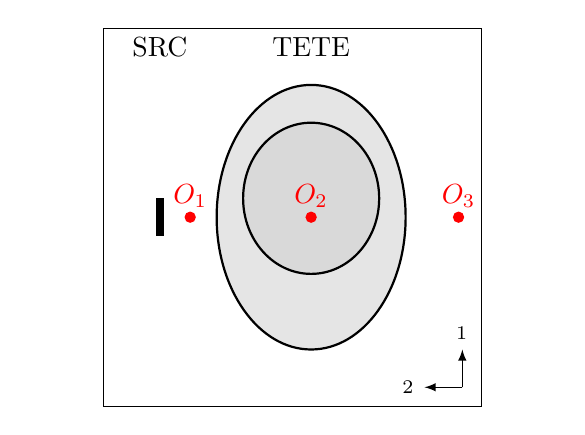
\begin{tikzpicture}[scale=4.8]
		\fill[white] (-0.2,0) rectangle (1.2,1);
		\draw (0,0) rectangle (1,1);
		\fill (0.14,0.45) rectangle (0.16,0.55);
		\draw[thick,fill=gray!20] (0.55,0.5) ellipse (0.25 and 0.35);
		\draw[thick,fill=gray!30] (0.55,0.55) ellipse (0.18 and 0.2);
		\draw (0.15,1) node[below] {SRC};
		\draw (0.55,1) node[below] {TETE};
		\draw[arrows={-latex}] (0.95,0.05) -- (0.95,0.15) node[above] {$\x_1$};
		\draw[arrows={-latex}] (0.95,0.05) -- (0.85,0.05) node[left] {$\x_2$};
		\fill[red] (0.23,0.5) circle (0.015) node[above,red]{$O_1$};
		\fill[red] (0.55,0.5) circle (0.015) node[above,red]{$O_2$};
		\fill[red] (0.94,0.5) circle (0.015) node[above,red]{$O_3$};
		\end{tikzpicture}
	}	
\end{figure}



\subsection{Application du schéma LRK2}
\label{ssect:tete_simplifiee_lrk2}

Avant d'appliquer la méthode à pas de temps local, nous commençons par appliquer
le schéma LRK$2$ décrit dans la section \ref{sect:pas de temps local lrk2}.
Rappelons qu'il s'agit du schéma RK$2$ modifié pour effectuer
une prédiction locale à chaque maille. L'étape de mise-à-jour reste inchangée.
Le pas de temps de simulation est homogène
sur tout le maillage et nous reprenons la condition CFL \eqref{eq:cfl1}.

Le coefficient CFL de ce schéma, déterminé par la méthode de la puissance
itérée pour l'ordre d'interpolation spatiale $\Deg=2$, est de $1.9$.
La stabilité de ce schéma est donc inférieure au schéma RK$2$.
Le pas de temps de la simulation est de $4.071 \cdot 10^{-14}$ s
et le temps de calcul sur NVidia GeForce GTX 1080 Ti est de $1.71$ heures.

Les résultats avec l'application de ce schéma sont équivalents à ceux obtenus
avec le schéma RK$2$, malgré l'utilisation d'un prédicteur local.
Cependant, cette méthode est $1.44$ fois moins efficace
compte tenu de son coefficient CFL de stabilité.
Remarquons tout de même qu'à pas de temps égal, ce schéma serait plus efficace
que le schéma RK$2$ de $12$ \%, cela grâce aux propiétés locales du terme de flux
de l'étape de prédiction.
\\


\subsection{Application du schéma LTS2}
\label{ssect:tete_simplifiee_dt_local}


Contrairement à une méthode à pas de temps homogène telle que
les méthodes de type RK (section \ref{ssect:rk}), le schéma LTS$2$ impose
de vérifier un critère de type CFL sur chaque maille.
Dans le cas d'une méthode à pas de temps homogène,
il suffit de satisfaire
la condition CFL sur la maille la plus
contraignante (généralement une seule maille : la plus petite, ou
dans certains cas une maille très déformée).

Une condition CFL de stabilité offrant les meilleurs performances
est donc difficile à déterminer. En effet, dans le cas d'une une grande
maille (déformée) sur laquelle le schéma en temps homogène était stable avec
le pas de temps imposé par la plus petite maille du maillage,
des instabilités peuvent apparaitre lors de l'utilisation d'un pas de
temps (calculé avec la même condition CFL) propre à chaque maille.

Nous présentons donc des résultats pour les coefficients CFL
de stabilité maximaux dans le cas de l'application des critères
CFL \eqref{eq:cfl1} et \eqref{eq:cfl2}.
Nous noterons respectivement ces critères CFL$1$ et CFL$2$.
Pour le second critère, nous avons testé différentes valeurs pour l'exposant $\alpha$.
Ce paramètre permet de faire varier le gradient de la fonction
qui associe à chaque maille son pas de temps et impacte directement
la répartition des classes de pas de temps qui utilise la fonction $\log_2$.
\\

Nous utilisons le schéma LTS$2$ sur le cas d'application de
l'antenne dipolaire placée à proximité d'une tête humaine simplifiée
(section \ref{ssect:tete_simplifiee_desc}).
Nous choisissons l'ordre d'interpolation spatiale $\Deg = 1$ et
remplaçons la condition de bord PML par la condition de
Silver-Müller (section \ref{ssect:silver_mueller}).
Dans ces conditions, la simulation à l'aide du schéma couplé GD-RK$2$
sur $20$ ns de temps physique a nécessité $0.44$ heures de calcul
sur un GPU NVidia GeForce GTX 1070.
Le pas de temps de cette simulation est de $1.446 \cdot 10^{-13}$ s
déterminé à l'aide du critère CFL \eqref{eq:cfl1}.
Le coefficient CFL de stabilité déterminé par la méthode
de la puissance itérée (section \ref{ssect:puissance itérée})
est de $4.5$.


\subsubsection{Mémoire}

Du point de vue de la mémoire, la simulation GD-RK$2$ occupe $142$ Mo sur le
GPU contre en moyenne $155$ Mo dans le cas des simulations GD-LTS$2$,
soit environ $10$ \% de plus de mémoire utile pour le schéma LTS$2$.

Cette faible différence d'occupation en mémoire est principalement liée à la
génération d'interfaces supplémentaires entre les classes de pas de temps
et les zones de mailles tampon.
En effet, l'implémentation actuelle de ce schéma utilise le découpage en zones homogènes
pour séparer les classes de pas de temps et les mailles tampon.


\subsubsection{Performances}


Les performances en dimension $3$ sont nettement inférieures à celles constatées en
dimension $1$ (section \ref{sect:pas de temps local transport}).
En effet, en dimension $1$, une interface (terme de flux) entre $2$ classes de pas de
temps ne représente qu'un seul degré de liberté contre des milliers en dimension $3$.
Ces interfaces sont des surfaces fermées topologiquement comparables à des
frontières de boules.

Dans le cas de la simulation à pas de temps homogène, toutes les mailles
sont regroupées en une unique zone homogène.
Les kernels de calcul sont donc peu nombreux et traitent un grand nombre
de mailles.
Dans le cas des simulations à pas de temps local, nous avons entre $6$ et $16$
zones homogènes supplémentaires, issues du découpage en classes de pas de temps.
Ce découpage multiplie d'autant le nombre de kernels exécutés et génère
une interface entre chacune de ces zones (agencement en « peau d'oignon »).
Ces zones et interfaces comptent un nombre de mailles réduit, les kernels sont donc
moins efficaces, en plus d'augmenter le temps de latence OpenCL
par leur nombre.

Néanmoins, malgré tous ces facteurs diminuant l'efficacité
en OpenCL et dimension $3$, nous avons obtenu
de meilleures performances en temps de calcul à l'aide du schéma LTS$2$.
Le tableau \ref{tab:lts2_perfs} présente les résultats en temps de calcul
en fonction du critère et du coefficient de CFL.

\begin{figure}[!h]
	\centering
	\caption{
		\label{tab:lts2_perfs}
		Temps de calcul des méthodes RK$2$ et LTS$2$ en fonction
		du critère et du coefficient de CFL sur GPU NVidia GeForce GTX 1070
		dans le cas de la simulation de l'antenne ELPOSD
		placée à proximité de la tête humaine simplifiée
		pour l'ordre d'interpolation spatiale $\Deg = 1$.
		La dernière ligne correspond au temps de calcul obtenu en prenant pour chaque
		maille le plus grand pas de temps donné par tous les critères CFL précédents.
		}
		
	\begin{tabular}{|c|c|c|c|c|c|c|}
		\hline
		\multirow{2}{*}{Méthode} & \multicolumn{3}{c|}{CFL} & \multirow{2}{*}{$\dt_{\min}^l$ (s)} & \multirow{2}{*}{$N_t$} & \multirow{2}{*}{$T_\mathrm{s}$ (h)} \\	\cline{2-4}
		& crit. & $\alpha$ & coeff. & & & \\	\hline\hline
		RK$2$ & $1$ & - & $4.5$ & $1.446 \cdot 10^{-13}$ & $0$ & $0.44$ \\ \hline
		\multirow{8}{*}{LTS$2$} & $1$ & - & $0.22$ & $7.070 \cdot 10^{-15}$ & $7$ & $1.10$ \\ \cline{2-7}
		& \multirow{6}{*}{$2$} & $4/3$ & $1.2 \cdot 10^{3}$ & $3.285 \cdot 10^{-15}$ & $8$ & $2.21$ \\ \cline{3-7}
		& & $1$ & $0.20$ & $8.601 \cdot 10^{-15}$ & $7$ & $0.96$ \\ \cline{3-7}
		& & $3/4$ & $3.2 \cdot 10^{-4}$ & $1.931 \cdot 10^{-14}$ & $6$ & $0.54$ \\ \cline{3-7}
		& & $2/3$ & $3.1 \cdot 10^{-5}$ & $2.094 \cdot 10^{-14}$ & $5$ & $0.50$ \\ \cline{3-7}
		& & $1/2$ & $4.5 \cdot 10^{-7}$ & $3.894 \cdot 10^{-14}$ & $4$ & $0.39$ \\ \cline{3-7}
		& & $1/4$ & $6.5 \cdot 10^{-10}$ & $7.721 \cdot 10^{-14}$ & $3$ & $0.33$ \\ \cline{2-7}
		& \multicolumn{3}{c|}{$\max \dt$} & $7.721 \cdot 10^{-14}$ & $4$ & $0.28$ \\ \hline
	\end{tabular}
\end{figure}


\begin{figure}[!h]
	\centering
	\caption{
		\label{tab:lts2_classes}
		Composition des zones homogènes pour les méthodes RK$2$ et LTS$2$ en fonction
		du critère et du coefficient de CFL
		dans le cas de la simulation de l'antenne ELPOSD
		placée à proximité de la tête humaine simplifiée
		pour l'ordre d'interpolation spatiale $\Deg = 1$.
	}
	
	\subfloat[Zones homogènes.]{
		\label{tab:lts2_classes_zones}
	\resizebox{0.85\linewidth}{!}{%
	\begin{tabular}{|c|c|c|c|c|c|c|c|c|c|}
		\hline
		\textbf{Méthode} & RK$2$ & \multicolumn{8}{c|}{LTS$2$} \\	\hline
		\textbf{CFL}[-$\alpha$] & $1$ & $1$ & $2$-$4/3$ & $2$-$1$ & $2$-$3/4$ & $2$-$2/3$ & $2$-$1/2$ & $2$-$1/4$ & $\max \dt$ \\	\hline\hline
		$N_t$ & $0$ & $7$ & $8$ & $7$ & $6$ & $5$ & $4$ & $3$ & $4$ \\ \hline\hline
		$\#\mathcal{C}_0$ \eqref{eq:lts2_classes} & $77652$ & $640$ & $601$ & $649$ & $799$ & $876$ & $1063$ & $4741$ & $4560$ \\	\hline
		$\#\mathcal{T}_0$ \eqref{eq:lts2_tampon} & - & $608$ & $592$ & $660$ & $593$ & $540$ & $527$ & $1552$ & $1603$ \\	\hline
		$\#\mathcal{C}_1\setminus\mathcal{T}_0$ & - & $1036$ & $1035$ & $975$ & $1289$ & $1422$ & $3239$ & $21551$ & $2414$ \\	\hline
		$\#\mathcal{T}_1$ & - & $984$ & $1016$ & $984$ & $1113$ & $1099$ & $1504$ & $2056$ & $2178$ \\	\hline
		$\#\mathcal{C}_2\setminus\mathcal{T}_1$ & - & $1156$ & $1128$ & $1167$ & $1749$ & $2812$ & $11063$ & $11169$ & $9941$ \\	\hline
		$\#\mathcal{T}_2$ & - & $1088$ & $1068$ & $1093$ & $1269$ & $1443$ & $4548$ & $5499$ & $11074$ \\	\hline
		$\#\mathcal{C}_3\setminus\mathcal{T}_2$ & - & $1208$ & $1065$ & $1262$ & $4843$ & $9403$ & $17074$ & $31084$ & $39058$ \\	\hline
		$\#\mathcal{T}_3$ & - & $1036$ & $924$ & $1045$ & $4352$ & $4682$ & $6204$ & - & $6608$ \\	\hline
		$\#\mathcal{C}_4\setminus\mathcal{T}_3$ & - & $1704$ & $833$ & $1779$ & $20045$ & $18492$ & $32430$ & - & $216$ \\	\hline
		$\#\mathcal{T}_4$ & - & $2224$ & $895$ & $2331$ & $7332$ & $5573$ & - & - & - \\	\hline
		$\#\mathcal{C}_5\setminus\mathcal{T}_4$ & - & $9888$ & $1147$ & $10259$ & $30144$ & $31310$ & - & - & - \\	\hline
		$\#\mathcal{T}_5$ & - & $9828$ & $1448$ & $10331$ & $4108$ & - & - & - & - \\	\hline
		$\#\mathcal{C}_6\setminus\mathcal{T}_5$ & - & $33384$ & $3455$ & $36614$ & $16$ & - & - & - & - \\	\hline
		$\#\mathcal{T}_6$ & - & $12476$ & $5734$ & $8443$ & - & - & - & - & - \\	\hline
		$\#\mathcal{C}_7\setminus\mathcal{T}_6$ & - & $392$ & $15980$ & $60$ & - & - & - & - & - \\	\hline
		$\#\mathcal{T}_7$ & - & - & $17203$ & - & - & - & - & - & - \\	\hline
		$\#\mathcal{C}_8\setminus\mathcal{T}_7$ & - & - & $23528$ & - & - & - & - & - & - \\	\hline
	\end{tabular}}
	}
	\\
	\subfloat[Interfaces.]{
		\label{tab:lts2_classes_interfaces}
	\resizebox{0.85\linewidth}{!}{%
	\begin{tabular}{|c|c|c|c|c|c|c|c|c|c|}
		\hline
		\textbf{Méthode} & RK$2$ & \multicolumn{8}{c|}{LTS$2$} \\	\hline
		\textbf{CFL}[-$\alpha$] & $1$ & $1$ & $2$-$4/3$ & $2$-$1$ & $2$-$3/4$ & $2$-$2/3$ & $2$-$1/2$ & $2$-$1/4$ & $\max \dt$ \\	\hline\hline
		$N_t$ & $0$ & $7$ & $8$ & $7$ & $6$ & $5$ & $4$ & $3$ & $4$ \\ \hline\hline
		$\#\mathcal{I}_0$ \eqref{eq:lts2_interfaces} & - & $570$ & $570$ & $580$ & $544$ & $486$ & $464$ & $1428$ & $1474$ \\	\hline
		$\#\Adh{\mathcal{T}_0} \cap \Adh{\mathcal{C}_1\setminus\mathcal{T}_0}$ & - & $582$ & $610$ & $544$ & $486$ & $474$ & $464$ & $1176$ & $1202$ \\	\hline
		$\#\mathcal{I}_1$ & - & $858$ & $900$ & $858$ & $992$ & $972$ & $1356$ & $1560$ & $1802$ \\	\hline
		$\#\Adh{\mathcal{T}_1} \cap \Adh{\mathcal{C}_2\setminus\mathcal{T}_1}$
		& - & $936$ & $966$ & $936$ & $1004$ & $992$ & $1152$ & $3168$ & $2584$ \\	\hline
		$\#\mathcal{I}_2$
		& - & $972$ & $966$ & $976$ & $1132$ & $1276$ & $3796$ & $4298$ & $9278$ \\	\hline
		$\#\Adh{\mathcal{T}_2} \cap \Adh{\mathcal{C}_3\setminus\mathcal{T}_2}$
		& - & $996$ & $1026$ & $1030$ & $1088$ & $1294$ & $5456$ & $5772$ & $9148$ \\	\hline
		$\#\mathcal{I}_3$
		& - & $978$ & $906$ & $1006$ & $3570$ & $3936$ & $5222$ & - & $7649$ \\	\hline
		$\#\Adh{\mathcal{T}_3} \cap \Adh{\mathcal{C}_4\setminus\mathcal{T}_3}$
		& - & $888$ & $790$ & $922$ & $4800$ & $5532$ & $6426$ & - & $309$ \\	\hline
		$\#\mathcal{I}_4$
		& - & $1872$ & $856$ & $2040$ & $6542$ & $4430$ & - & - & - \\	\hline
		$\#\Adh{\mathcal{T}_4} \cap \Adh{\mathcal{C}_5\setminus\mathcal{T}_4}$
		& - & $2910$ & $1002$ & $3048$ & $6654$ & $6270$ & - & - & - \\	\hline
		$\#\mathcal{I}_5$
		& - & $8172$ & $1326$ & $8522$ & $4998$ & - & - & - & - \\	\hline
		$\#\Adh{\mathcal{T}_5} \cap \Adh{\mathcal{C}_6\setminus\mathcal{T}_5}$
		& - & $9132$ & $1820$ & $9434$ & $24$ & - & - & - & - \\	\hline
		$\#\mathcal{I}_6$
		& - & $12028$ & $4831$ & $8994$ & - & - & - & - & - \\	\hline
		$\#\Adh{\mathcal{T}_6} \cap \Adh{\mathcal{C}_7\setminus\mathcal{T}_6}$
		& - & $480$ & $7101$ & $66$ & - & - & - & - & - \\	\hline
		$\#\mathcal{I}_7$
		& - & - & $13042$ & - & - & - & - & - & - \\	\hline
		$\#\Adh{\mathcal{T}_7} \cap \Adh{\mathcal{C}_8\setminus\mathcal{T}_7}$
		& - & - & $13504$ & - & - & - & - & - & - \\	\hline
	\end{tabular}}
	}
\end{figure}


Nous pouvons constater qu'avec un bon critère CFL, le pas de temps de
stabilité du schéma LTS$2$ est seulement $2$ fois plus petit
que celui du schéma RK$2$.
Nous observons aussi que les meilleures performances ne sont pas obtenues
avec le plus grand nombre de classes de pas de temps. Rappelons que
le nombre de classes de pas de temps augmente la quantité de kernels
et le nombre d'interfaces.
Le nombre de mailles par classe de pas de temps et par interface est donné dans le
tableau \ref{tab:lts2_classes}.

Du point de vue de la répartition des classes de pas de temps, le cas « $\max\dt$ »
est très proche de celui pour lequel nous appliquons le critère CFL$2$ avec le
paramètre $\alpha=1/4$. La principale différence réside dans le fait que
l'utilisation du pas de temps maximal de toutes les conditions CFL précédentes
déplace un certain nombre de mailles dans les classes supérieures.

Puisque la classe $\mathcal{C}_0$ contient très peu de mailles dans le cas « $\max\dt$ »,
nous avons relancé la simulation en imposant le maximum de $N_t=3$ dans le
but de réduire le nombre de kernels.
Suite à cette modification, le gain de performances constaté est de $2.77$ \%.
Ce gain peut paraître faible, mais n'a nécessité que très peu d'efforts.
\\




% ordre 1
% bords SM
% max cfl 0,28377472 h
%2018-07-26 13:23:11, info| Time scheme: ADER LOCAL AFLL
%2018-07-26 13:23:11, info| Starting time: 0s
%2018-07-26 13:23:11, info| Final time: 2e-08s
%2018-07-26 13:23:11, info| Number of iteration: 16190
%2018-07-26 13:23:11, info| Min time step: 7.72101e-14s
%2018-07-26 13:23:11, info| Max time step: 1.23536e-12s
%2018-07-26 13:23:11, info| Number of steps per iter: 16
%2018-07-26 13:23:11, info| Composition of the simulation:
%2018-07-26 13:23:11, info|   zone 0: 4560 element(s) of order 1 (level: 0).
%2018-07-26 13:23:11, info|   zone 1: 1603 element(s) of order 1 (level: 0.5).
%2018-07-26 13:23:11, info|   zone 2: 2414 element(s) of order 1 (level: 1).
%2018-07-26 13:23:11, info|   zone 3: 2178 element(s) of order 1 (level: 1.5).
%2018-07-26 13:23:11, info|   zone 4: 9941 element(s) of order 1 (level: 2).
%2018-07-26 13:23:11, info|   zone 5: 11074 element(s) of order 1 (level: 2.5).
%2018-07-26 13:23:11, info|   zone 6: 39058 element(s) of order 1 (level: 3).
%2018-07-26 13:23:11, info|   zone 7: 6608 element(s) of order 1 (level: 3.5).
%2018-07-26 13:23:11, info|   zone 8: 216 element(s) of order 1 (level: 4).
%2018-07-26 13:23:11, info|   interface 9 between zone 0 and zone 1: 1474 element(s) (ref: 1/1, group size: 1/1, nb set of groups: 6).
%2018-07-26 13:23:11, info|   interface 10 between zone 1 and zone 2: 1202 element(s) (ref: 1/1, group size: 1/1, nb set of groups: 5).
%2018-07-26 13:23:11, info|   interface 11 between zone 2 and zone 3: 1802 element(s) (ref: 1/1, group size: 1/1, nb set of groups: 7).
%2018-07-26 13:23:11, info|   interface 12 between zone 3 and zone 4: 2584 element(s) (ref: 1/1, group size: 1/1, nb set of groups: 6).
%2018-07-26 13:23:11, info|   interface 13 between zone 4 and zone 5: 9278 element(s) (ref: 1/1, group size: 1/1, nb set of groups: 6).
%2018-07-26 13:23:11, info|   interface 14 between zone 5 and zone 6: 9148 element(s) (ref: 1/1, group size: 1/1, nb set of groups: 5).
%2018-07-26 13:23:11, info|   interface 15 between zone 6 and zone 7: 7649 element(s) (ref: 1/1, group size: 1/1, nb set of groups: 6).
%2018-07-26 13:23:11, info|   interface 17 between zone 7 and zone 8: 309 element(s) (ref: 1/1, group size: 1/1, nb set of groups: 5).
%2018-07-26 13:23:11, info|  Number of volumic elements: 77652.
%2018-07-26 13:23:11, info| Memory allocated on the computational unit: 154Mo 2ko 736o


% ordre 1
% bords SM
% cfl2 alpha = 0.25 coeff 0.00000000065
% temps : 0,325598 h
%2018-07-26 12:41:14, info| Time scheme: ADER LOCAL AFLL
%2018-07-26 12:41:14, info| Starting time: 0s
%2018-07-26 12:41:14, info| Final time: 2e-08s
%2018-07-26 12:41:14, info| Number of iteration: 32380
%2018-07-26 12:41:14, info| Min time step: 7.72101e-14s
%2018-07-26 12:41:14, info| Max time step: 6.1768e-13s
%2018-07-26 12:41:14, info| Number of steps per iter: 8
%2018-07-26 12:41:14, info| Composition of the simulation:
%2018-07-26 12:41:14, info|   zone 0: 4741 element(s) of order 1 (level: 0).
%2018-07-26 12:41:14, info|   zone 1: 1552 element(s) of order 1 (level: 0.5).
%2018-07-26 12:41:14, info|   zone 2: 21551 element(s) of order 1 (level: 1).
%2018-07-26 12:41:14, info|   zone 3: 2056 element(s) of order 1 (level: 1.5).
%2018-07-26 12:41:14, info|   zone 4: 11169 element(s) of order 1 (level: 2).
%2018-07-26 12:41:14, info|   zone 5: 5499 element(s) of order 1 (level: 2.5).
%2018-07-26 12:41:14, info|   zone 6: 31084 element(s) of order 1 (level: 3).
%2018-07-26 12:41:14, info|   interface 7 between zone 0 and zone 1: 1428 element(s) (ref: 1/1, group size: 1/1, nb set of groups: 6).
%2018-07-26 12:41:14, info|   interface 8 between zone 1 and zone 2: 1176 element(s) (ref: 1/1, group size: 1/1, nb set of groups: 5).
%2018-07-26 12:41:14, info|   interface 10 between zone 2 and zone 3: 1560 element(s) (ref: 1/1, group size: 1/1, nb set of groups: 2).
%2018-07-26 12:41:14, info|   interface 11 between zone 3 and zone 4: 3168 element(s) (ref: 1/1, group size: 1/1, nb set of groups: 3).
%2018-07-26 12:41:14, info|   interface 12 between zone 4 and zone 5: 4298 element(s) (ref: 1/1, group size: 1/1, nb set of groups: 6).
%2018-07-26 12:41:14, info|   interface 13 between zone 5 and zone 6: 5772 element(s) (ref: 1/1, group size: 1/1, nb set of groups: 3).
%2018-07-26 12:41:14, info|  Number of volumic elements: 77652.
%2018-07-26 12:41:14, info| Memory allocated on the computational unit: 147Mo 581ko 536o


% ordre 1
% bords SM
% cfl2 alpha = 0.5 coeff 0.00000046
% temps : 0,3887545 h
%2018-07-26 11:23:33, info| Time scheme: ADER LOCAL AFLL
%2018-07-26 11:23:33, info| Starting time: 0s
%2018-07-26 11:23:33, info| Final time: 2e-08s
%2018-07-26 11:23:33, info| Number of iteration: 32099
%2018-07-26 11:23:33, info| Min time step: 3.89431e-14s
%2018-07-26 11:23:33, info| Max time step: 6.23089e-13s
%2018-07-26 11:23:33, info| Number of steps per iter: 16
%2018-07-26 11:23:33, info| Composition of the simulation:
%2018-07-26 11:23:33, info|   zone 0: 1063 element(s) of order 1 (level: 0).
%2018-07-26 11:23:33, info|   zone 1: 527 element(s) of order 1 (level: 0.5).
%2018-07-26 11:23:33, info|   zone 2: 3239 element(s) of order 1 (level: 1).
%2018-07-26 11:23:33, info|   zone 3: 1504 element(s) of order 1 (level: 1.5).
%2018-07-26 11:23:33, info|   zone 4: 11063 element(s) of order 1 (level: 2).
%2018-07-26 11:23:33, info|   zone 5: 4548 element(s) of order 1 (level: 2.5).
%2018-07-26 11:23:33, info|   zone 6: 17074 element(s) of order 1 (level: 3).
%2018-07-26 11:23:33, info|   zone 7: 6204 element(s) of order 1 (level: 3.5).
%2018-07-26 11:23:33, info|   zone 8: 32430 element(s) of order 1 (level: 4).
%2018-07-26 11:23:33, info|   interface 9 between zone 0 and zone 1: 464 element(s) (ref: 1/1, group size: 1/1, nb set of groups: 6).
%2018-07-26 11:23:33, info|   interface 10 between zone 1 and zone 2: 464 element(s) (ref: 1/1, group size: 1/1, nb set of groups: 5).
%2018-07-26 11:23:33, info|   interface 11 between zone 2 and zone 3: 1356 element(s) (ref: 1/1, group size: 1/1, nb set of groups: 6).
%2018-07-26 11:23:33, info|   interface 12 between zone 3 and zone 4: 1152 element(s) (ref: 1/1, group size: 1/1, nb set of groups: 5).
%2018-07-26 11:23:33, info|   interface 13 between zone 4 and zone 5: 3796 element(s) (ref: 1/1, group size: 1/1, nb set of groups: 6).
%2018-07-26 11:23:33, info|   interface 15 between zone 5 and zone 6: 5456 element(s) (ref: 1/1, group size: 1/1, nb set of groups: 5).
%2018-07-26 11:23:33, info|   interface 17 between zone 6 and zone 7: 5222 element(s) (ref: 1/1, group size: 1/1, nb set of groups: 6).
%2018-07-26 11:23:33, info|   interface 18 between zone 7 and zone 8: 6426 element(s) (ref: 1/1, group size: 1/1, nb set of groups: 5).
%2018-07-26 11:23:33, info|  Number of volumic elements: 77652.
%2018-07-26 11:23:33, info| Memory allocated on the computational unit: 150Mo 84ko 780o



% ordre 1
% bords SM
% cfl2 alpha = 0.66666 coeff 0.000031
% temps : 0,5032704 h
%2018-07-26 10:32:24, info| Time scheme: ADER LOCAL AFLL
%2018-07-26 10:32:24, info| Starting time: 0s
%2018-07-26 10:32:24, info| Final time: 2e-08s
%2018-07-26 10:32:24, info| Number of iteration: 29848
%2018-07-26 10:32:24, info| Min time step: 2.09399e-14s
%2018-07-26 10:32:24, info| Max time step: 6.70078e-13s
%2018-07-26 10:32:24, info| Number of steps per iter: 32
%2018-07-26 10:32:24, info| Composition of the simulation:
%2018-07-26 10:32:24, info|   zone 0: 876 element(s) of order 1 (level: 0).
%2018-07-26 10:32:24, info|   zone 1: 540 element(s) of order 1 (level: 0.5).
%2018-07-26 10:32:24, info|   zone 2: 1422 element(s) of order 1 (level: 1).
%2018-07-26 10:32:24, info|   zone 3: 1099 element(s) of order 1 (level: 1.5).
%2018-07-26 10:32:24, info|   zone 4: 2812 element(s) of order 1 (level: 2).
%2018-07-26 10:32:24, info|   zone 5: 1443 element(s) of order 1 (level: 2.5).
%2018-07-26 10:32:24, info|   zone 6: 9403 element(s) of order 1 (level: 3).
%2018-07-26 10:32:24, info|   zone 7: 4682 element(s) of order 1 (level: 3.5).
%2018-07-26 10:32:24, info|   zone 8: 18492 element(s) of order 1 (level: 4).
%2018-07-26 10:32:24, info|   zone 9: 5573 element(s) of order 1 (level: 4.5).
%2018-07-26 10:32:24, info|   zone 10: 31310 element(s) of order 1 (level: 5).
%2018-07-26 10:32:24, info|   interface 11 between zone 0 and zone 1: 486 element(s) (ref: 1/1, group size: 1/1, nb set of groups: 3).
%2018-07-26 10:32:24, info|   interface 12 between zone 1 and zone 2: 474 element(s) (ref: 1/1, group size: 1/1, nb set of groups: 3).
%2018-07-26 10:32:24, info|   interface 13 between zone 2 and zone 3: 972 element(s) (ref: 1/1, group size: 1/1, nb set of groups: 6).
%2018-07-26 10:32:24, info|   interface 14 between zone 3 and zone 4: 992 element(s) (ref: 1/1, group size: 1/1, nb set of groups: 5).
%2018-07-26 10:32:24, info|   interface 15 between zone 4 and zone 5: 1276 element(s) (ref: 1/1, group size: 1/1, nb set of groups: 6).
%2018-07-26 10:32:24, info|   interface 16 between zone 5 and zone 6: 1294 element(s) (ref: 1/1, group size: 1/1, nb set of groups: 5).
%2018-07-26 10:32:24, info|   interface 17 between zone 6 and zone 7: 3936 element(s) (ref: 1/1, group size: 1/1, nb set of groups: 6).
%2018-07-26 10:32:24, info|   interface 19 between zone 7 and zone 8: 5532 element(s) (ref: 1/1, group size: 1/1, nb set of groups: 5).
%2018-07-26 10:32:24, info|   interface 21 between zone 8 and zone 9: 4430 element(s) (ref: 1/1, group size: 1/1, nb set of groups: 6).
%2018-07-26 10:32:24, info|   interface 22 between zone 9 and zone 10: 6270 element(s) (ref: 1/1, group size: 1/1, nb set of groups: 6).
%2018-07-26 10:32:24, info|  Number of volumic elements: 77652.
%2018-07-26 10:32:24, info| Memory allocated on the computational unit: 150Mo 553ko 856o


% ordre 1
% bords SM
% cfl2 alpha = 0.75 coeff 0.00032
% temps : 0,5350372 h
%2018-07-25 14:22:35, info| Time scheme: ADER LOCAL AFLL
%2018-07-25 14:22:35, info| Starting time: 0s
%2018-07-25 14:22:35, info| Final time: 2e-08s
%2018-07-25 14:22:35, info| Number of iteration: 16186
%2018-07-25 14:22:35, info| Min time step: 1.93079e-14s
%2018-07-25 14:22:35, info| Max time step: 1.2357e-12s
%2018-07-25 14:22:35, info| Number of steps per iter: 64
%2018-07-25 14:22:35, info| Composition of the simulation:
%2018-07-25 14:22:35, info|   zone 0: 799 element(s) of order 1 (level: 0).
%2018-07-25 14:22:35, info|   zone 1: 593 element(s) of order 1 (level: 0.5).
%2018-07-25 14:22:35, info|   zone 2: 1289 element(s) of order 1 (level: 1).
%2018-07-25 14:22:35, info|   zone 3: 1113 element(s) of order 1 (level: 1.5).
%2018-07-25 14:22:35, info|   zone 4: 1749 element(s) of order 1 (level: 2).
%2018-07-25 14:22:35, info|   zone 5: 1269 element(s) of order 1 (level: 2.5).
%2018-07-25 14:22:35, info|   zone 6: 4843 element(s) of order 1 (level: 3).
%2018-07-25 14:22:35, info|   zone 7: 4352 element(s) of order 1 (level: 3.5).
%2018-07-25 14:22:35, info|   zone 8: 20045 element(s) of order 1 (level: 4).
%2018-07-25 14:22:35, info|   zone 9: 7332 element(s) of order 1 (level: 4.5).
%2018-07-25 14:22:35, info|   zone 10: 30144 element(s) of order 1 (level: 5).
%2018-07-25 14:22:35, info|   zone 11: 4108 element(s) of order 1 (level: 5.5).
%2018-07-25 14:22:35, info|   zone 12: 16 element(s) of order 1 (level: 6).
%2018-07-25 14:22:35, info|   interface 13 between zone 0 and zone 1: 544 element(s) (ref: 1/1, group size: 1/1, nb set of groups: 6).
%2018-07-25 14:22:35, info|   interface 14 between zone 1 and zone 2: 486 element(s) (ref: 1/1, group size: 1/1, nb set of groups: 3).
%2018-07-25 14:22:35, info|   interface 15 between zone 2 and zone 3: 992 element(s) (ref: 1/1, group size: 1/1, nb set of groups: 5).
%2018-07-25 14:22:35, info|   interface 16 between zone 3 and zone 4: 1004 element(s) (ref: 1/1, group size: 1/1, nb set of groups: 5).
%2018-07-25 14:22:35, info|   interface 17 between zone 4 and zone 5: 1132 element(s) (ref: 1/1, group size: 1/1, nb set of groups: 5).
%2018-07-25 14:22:35, info|   interface 18 between zone 5 and zone 6: 1088 element(s) (ref: 1/1, group size: 1/1, nb set of groups: 5).
%2018-07-25 14:22:35, info|   interface 19 between zone 6 and zone 7: 3570 element(s) (ref: 1/1, group size: 1/1, nb set of groups: 6).
%2018-07-25 14:22:35, info|   interface 20 between zone 7 and zone 8: 4800 element(s) (ref: 1/1, group size: 1/1, nb set of groups: 5).
%2018-07-25 14:22:35, info|   interface 22 between zone 8 and zone 9: 6542 element(s) (ref: 1/1, group size: 1/1, nb set of groups: 6).
%2018-07-25 14:22:35, info|   interface 23 between zone 9 and zone 10: 6654 element(s) (ref: 1/1, group size: 1/1, nb set of groups: 5).
%2018-07-25 14:22:35, info|   interface 24 between zone 10 and zone 11: 4998 element(s) (ref: 1/1, group size: 1/1, nb set of groups: 6).
%2018-07-25 14:22:35, info|   interface 25 between zone 11 and zone 12: 24 element(s) (ref: 1/1, group size: 1/1, nb set of groups: 2).
%2018-07-25 14:22:35, info|  Number of volumic elements: 77652.
%2018-07-25 14:22:35, info| Memory allocated on the computational unit: 153Mo 166ko 64o


% ordre 1
% bords SM
% cfl2 alpha = 1 coeff 0.20
% temps : 0,958866 h
%2018-07-25 10:06:17, info| Time scheme: ADER LOCAL AFLL
%2018-07-25 10:06:17, info| Starting time: 0s
%2018-07-25 10:06:17, info| Final time: 2e-08s
%2018-07-25 10:06:17, info| Number of iteration: 18168
%2018-07-25 10:06:17, info| Min time step: 8.60054e-15s
%2018-07-25 10:06:17, info| Max time step: 1.10087e-12s
%2018-07-25 10:06:17, info| Number of steps per iter: 128
%2018-07-25 10:06:17, info| Composition of the simulation:
%2018-07-25 10:06:17, info|   zone 0: 649 element(s) of order 1 (level: 0).
%2018-07-25 10:06:17, info|   zone 1: 660 element(s) of order 1 (level: 0.5).
%2018-07-25 10:06:17, info|   zone 2: 975 element(s) of order 1 (level: 1).
%2018-07-25 10:06:17, info|   zone 3: 984 element(s) of order 1 (level: 1.5).
%2018-07-25 10:06:17, info|   zone 4: 1167 element(s) of order 1 (level: 2).
%2018-07-25 10:06:17, info|   zone 5: 1093 element(s) of order 1 (level: 2.5).
%2018-07-25 10:06:17, info|   zone 6: 1262 element(s) of order 1 (level: 3).
%2018-07-25 10:06:17, info|   zone 7: 1045 element(s) of order 1 (level: 3.5).
%2018-07-25 10:06:17, info|   zone 8: 1779 element(s) of order 1 (level: 4).
%2018-07-25 10:06:17, info|   zone 9: 2331 element(s) of order 1 (level: 4.5).
%2018-07-25 10:06:17, info|   zone 10: 10259 element(s) of order 1 (level: 5).
%2018-07-25 10:06:17, info|   zone 11: 10331 element(s) of order 1 (level: 5.5).
%2018-07-25 10:06:17, info|   zone 12: 36614 element(s) of order 1 (level: 6).
%2018-07-25 10:06:17, info|   zone 13: 8443 element(s) of order 1 (level: 6.5).
%2018-07-25 10:06:17, info|   zone 14: 60 element(s) of order 1 (level: 7).
%2018-07-25 10:06:17, info|   interface 15 between zone 0 and zone 1: 580 element(s) (ref: 1/1, group size: 1/1, nb set of groups: 6).
%2018-07-25 10:06:17, info|   interface 16 between zone 1 and zone 2: 544 element(s) (ref: 1/1, group size: 1/1, nb set of groups: 5).
%2018-07-25 10:06:17, info|   interface 17 between zone 2 and zone 3: 858 element(s) (ref: 1/1, group size: 1/1, nb set of groups: 3).
%2018-07-25 10:06:17, info|   interface 18 between zone 3 and zone 4: 936 element(s) (ref: 1/1, group size: 1/1, nb set of groups: 3).
%2018-07-25 10:06:17, info|   interface 19 between zone 4 and zone 5: 976 element(s) (ref: 1/1, group size: 1/1, nb set of groups: 6).
%2018-07-25 10:06:17, info|   interface 20 between zone 5 and zone 6: 1030 element(s) (ref: 1/1, group size: 1/1, nb set of groups: 5).
%2018-07-25 10:06:17, info|   interface 21 between zone 6 and zone 7: 1006 element(s) (ref: 1/1, group size: 1/1, nb set of groups: 5).
%2018-07-25 10:06:17, info|   interface 22 between zone 7 and zone 8: 922 element(s) (ref: 1/1, group size: 1/1, nb set of groups: 5).
%2018-07-25 10:06:17, info|   interface 23 between zone 8 and zone 9: 2040 element(s) (ref: 1/1, group size: 1/1, nb set of groups: 6).
%2018-07-25 10:06:17, info|   interface 24 between zone 9 and zone 10: 3048 element(s) (ref: 1/1, group size: 1/1, nb set of groups: 6).
%2018-07-25 10:06:17, info|   interface 25 between zone 10 and zone 11: 8522 element(s) (ref: 1/1, group size: 1/1, nb set of groups: 6).
%2018-07-25 10:06:17, info|   interface 27 between zone 11 and zone 12: 9434 element(s) (ref: 1/1, group size: 1/1, nb set of groups: 5).
%2018-07-25 10:06:17, info|   interface 29 between zone 12 and zone 13: 8994 element(s) (ref: 1/1, group size: 1/1, nb set of groups: 6).
%2018-07-25 10:06:17, info|   interface 30 between zone 13 and zone 14: 66 element(s) (ref: 1/1, group size: 1/1, nb set of groups: 2).
%2018-07-25 10:06:17, info|  Number of volumic elements: 77652.
%2018-07-25 10:06:17, info| Memory allocated on the computational unit: 155Mo 994ko 452o

% ordre 1
% bords SM
% cfl2 alpha = 4/3 coeff 1200
% temps : 2,2130472 h
%2018-07-25 11:23:27, info| Time scheme: ADER LOCAL AFLL
%2018-07-25 11:23:27, info| Starting time: 0s
%2018-07-25 11:23:27, info| Final time: 2e-08s
%2018-07-25 11:23:27, info| Number of iteration: 23782
%2018-07-25 11:23:27, info| Min time step: 3.28518e-15s
%2018-07-25 11:23:27, info| Max time step: 8.41007e-13s
%2018-07-25 11:23:27, info| Number of steps per iter: 256
%2018-07-25 11:23:27, info| Composition of the simulation:
%2018-07-25 11:23:27, info|   zone 0: 601 element(s) of order 1 (level: 0).
%2018-07-25 11:23:27, info|   zone 1: 592 element(s) of order 1 (level: 0.5).
%2018-07-25 11:23:27, info|   zone 2: 1035 element(s) of order 1 (level: 1).
%2018-07-25 11:23:27, info|   zone 3: 1016 element(s) of order 1 (level: 1.5).
%2018-07-25 11:23:27, info|   zone 4: 1128 element(s) of order 1 (level: 2).
%2018-07-25 11:23:27, info|   zone 5: 1068 element(s) of order 1 (level: 2.5).
%2018-07-25 11:23:27, info|   zone 6: 1065 element(s) of order 1 (level: 3).
%2018-07-25 11:23:27, info|   zone 7: 924 element(s) of order 1 (level: 3.5).
%2018-07-25 11:23:27, info|   zone 8: 833 element(s) of order 1 (level: 4).
%2018-07-25 11:23:27, info|   zone 9: 895 element(s) of order 1 (level: 4.5).
%2018-07-25 11:23:27, info|   zone 10: 1147 element(s) of order 1 (level: 5).
%2018-07-25 11:23:27, info|   zone 11: 1448 element(s) of order 1 (level: 5.5).
%2018-07-25 11:23:27, info|   zone 12: 3455 element(s) of order 1 (level: 6).
%2018-07-25 11:23:27, info|   zone 13: 5734 element(s) of order 1 (level: 6.5).
%2018-07-25 11:23:27, info|   zone 14: 15980 element(s) of order 1 (level: 7).
%2018-07-25 11:23:27, info|   zone 15: 17203 element(s) of order 1 (level: 7.5).
%2018-07-25 11:23:27, info|   zone 16: 23528 element(s) of order 1 (level: 8).
%2018-07-25 11:23:27, info|   interface 17 between zone 0 and zone 1: 570 element(s) (ref: 1/1, group size: 1/1, nb set of groups: 6).
%2018-07-25 11:23:27, info|   interface 18 between zone 1 and zone 2: 610 element(s) (ref: 1/1, group size: 1/1, nb set of groups: 5).
%2018-07-25 11:23:27, info|   interface 19 between zone 2 and zone 3: 900 element(s) (ref: 1/1, group size: 1/1, nb set of groups: 3).
%2018-07-25 11:23:27, info|   interface 20 between zone 3 and zone 4: 966 element(s) (ref: 1/1, group size: 1/1, nb set of groups: 3).
%2018-07-25 11:23:27, info|   interface 21 between zone 4 and zone 5: 966 element(s) (ref: 1/1, group size: 1/1, nb set of groups: 3).
%2018-07-25 11:23:27, info|   interface 22 between zone 5 and zone 6: 1026 element(s) (ref: 1/1, group size: 1/1, nb set of groups: 3).
%2018-07-25 11:23:27, info|   interface 23 between zone 6 and zone 7: 906 element(s) (ref: 1/1, group size: 1/1, nb set of groups: 6).
%2018-07-25 11:23:27, info|   interface 24 between zone 7 and zone 8: 790 element(s) (ref: 1/1, group size: 1/1, nb set of groups: 5).
%2018-07-25 11:23:27, info|   interface 25 between zone 8 and zone 9: 856 element(s) (ref: 1/1, group size: 1/1, nb set of groups: 6).
%2018-07-25 11:23:27, info|   interface 26 between zone 9 and zone 10: 1002 element(s) (ref: 1/1, group size: 1/1, nb set of groups: 5).
%2018-07-25 11:23:27, info|   interface 27 between zone 10 and zone 11: 1326 element(s) (ref: 1/1, group size: 1/1, nb set of groups: 6).
%2018-07-25 11:23:27, info|   interface 29 between zone 11 and zone 12: 1820 element(s) (ref: 1/1, group size: 1/1, nb set of groups: 5).
%2018-07-25 11:23:27, info|   interface 30 between zone 12 and zone 13: 4831 element(s) (ref: 1/1, group size: 1/1, nb set of groups: 6).
%2018-07-25 11:23:27, info|   interface 32 between zone 13 and zone 14: 7101 element(s) (ref: 1/1, group size: 1/1, nb set of groups: 6).
%2018-07-25 11:23:27, info|   interface 33 between zone 14 and zone 15: 13042 element(s) (ref: 1/1, group size: 1/1, nb set of groups: 6).
%2018-07-25 11:23:27, info|   interface 35 between zone 15 and zone 16: 13504 element(s) (ref: 1/1, group size: 1/1, nb set of groups: 6).
%2018-07-25 11:23:27, info|  Number of volumic elements: 77652.
%2018-07-25 11:23:27, info| Memory allocated on the computational unit: 159Mo 726ko 624o


% ordre 1
% bords SM
% cfl 1 coeff 0.22
% temps : 1,09891083 h
%2018-07-25 15:13:04, info| Time scheme: ADER LOCAL AFLL
%2018-07-25 15:13:04, info| Starting time: 0s
%2018-07-25 15:13:04, info| Final time: 2e-08s
%2018-07-25 15:13:04, info| Number of iteration: 22101
%2018-07-25 15:13:04, info| Min time step: 7.06991e-15s
%2018-07-25 15:13:04, info| Max time step: 9.04949e-13s
%2018-07-25 15:13:04, info| Number of steps per iter: 128
%2018-07-25 15:13:04, info| Composition of the simulation:
%2018-07-25 15:13:04, info|   zone 0: 640 element(s) of order 1 (level: 0).
%2018-07-25 15:13:04, info|   zone 1: 608 element(s) of order 1 (level: 0.5).
%2018-07-25 15:13:04, info|   zone 2: 1036 element(s) of order 1 (level: 1).
%2018-07-25 15:13:04, info|   zone 3: 984 element(s) of order 1 (level: 1.5).
%2018-07-25 15:13:04, info|   zone 4: 1156 element(s) of order 1 (level: 2).
%2018-07-25 15:13:04, info|   zone 5: 1088 element(s) of order 1 (level: 2.5).
%2018-07-25 15:13:04, info|   zone 6: 1208 element(s) of order 1 (level: 3).
%2018-07-25 15:13:04, info|   zone 7: 1036 element(s) of order 1 (level: 3.5).
%2018-07-25 15:13:04, info|   zone 8: 1704 element(s) of order 1 (level: 4).
%2018-07-25 15:13:04, info|   zone 9: 2224 element(s) of order 1 (level: 4.5).
%2018-07-25 15:13:04, info|   zone 10: 9888 element(s) of order 1 (level: 5).
%2018-07-25 15:13:04, info|   zone 11: 9828 element(s) of order 1 (level: 5.5).
%2018-07-25 15:13:04, info|   zone 12: 33384 element(s) of order 1 (level: 6).
%2018-07-25 15:13:04, info|   zone 13: 12476 element(s) of order 1 (level: 6.5).
%2018-07-25 15:13:04, info|   zone 14: 392 element(s) of order 1 (level: 7).
%2018-07-25 15:13:04, info|   interface 15 between zone 0 and zone 1: 570 element(s) (ref: 1/1, group size: 1/1, nb set of groups: 3).
%2018-07-25 15:13:04, info|   interface 16 between zone 1 and zone 2: 582 element(s) (ref: 1/1, group size: 1/1, nb set of groups: 3).
%2018-07-25 15:13:04, info|   interface 17 between zone 2 and zone 3: 858 element(s) (ref: 1/1, group size: 1/1, nb set of groups: 3).
%2018-07-25 15:13:04, info|   interface 18 between zone 3 and zone 4: 936 element(s) (ref: 1/1, group size: 1/1, nb set of groups: 3).
%2018-07-25 15:13:04, info|   interface 19 between zone 4 and zone 5: 972 element(s) (ref: 1/1, group size: 1/1, nb set of groups: 3).
%2018-07-25 15:13:04, info|   interface 20 between zone 5 and zone 6: 996 element(s) (ref: 1/1, group size: 1/1, nb set of groups: 3).
%2018-07-25 15:13:04, info|   interface 21 between zone 6 and zone 7: 978 element(s) (ref: 1/1, group size: 1/1, nb set of groups: 3).
%2018-07-25 15:13:04, info|   interface 22 between zone 7 and zone 8: 888 element(s) (ref: 1/1, group size: 1/1, nb set of groups: 3).
%2018-07-25 15:13:04, info|   interface 23 between zone 8 and zone 9: 1872 element(s) (ref: 1/1, group size: 1/1, nb set of groups: 4).
%2018-07-25 15:13:04, info|   interface 24 between zone 9 and zone 10: 2910 element(s) (ref: 1/1, group size: 1/1, nb set of groups: 3).
%2018-07-25 15:13:04, info|   interface 25 between zone 10 and zone 11: 8172 element(s) (ref: 1/1, group size: 1/1, nb set of groups: 4).
%2018-07-25 15:13:04, info|   interface 27 between zone 11 and zone 12: 9132 element(s) (ref: 1/1, group size: 1/1, nb set of groups: 4).
%2018-07-25 15:13:04, info|   interface 29 between zone 12 and zone 13: 12028 element(s) (ref: 1/1, group size: 1/1, nb set of groups: 5).
%2018-07-25 15:13:04, info|   interface 30 between zone 13 and zone 14: 480 element(s) (ref: 1/1, group size: 1/1, nb set of groups: 3).
%2018-07-25 15:13:04, info|  Number of volumic elements: 77652.
%2018-07-25 15:13:04, info| Memory allocated on the computational unit: 156Mo 995ko 428o



%ordre 1 sans PML 0,44 h
%Time scheme: RK2
%2018-07-24 14:29:05, info| Starting time: 0s
%2018-07-24 14:29:05, info| Final time: 2e-08s
%2018-07-24 14:29:05, info| Number of iteration: 138301
%2018-07-24 14:29:05, info| Min time step: 1.44612e-13s
%2018-07-24 14:29:05, info| Max time step: 1.44612e-13s
%2018-07-24 14:29:05, info| Number of steps per iter: 1






\begin{figure}[!h]
	\centering
	\caption{
		\label{tab:lts2_ratios}
		Temps de calcul par kernel des méthodes RK$2$ et LTS$2$ (cas «~$\max\dt$~»)
		sur GPU NVidia GeForce GTX 1070
		dans le cas de la simulation de l'antenne ELPOSD
		placée à proximité de la tête humaine simplifiée
		pour l'ordre d'interpolation spatiale $\Deg = 1$
		sur $0.1$ ns de temps physique.
	}
	
	\begin{tabular}{|c|c|c|c|c|}
		\hline
		\multirow{2}{*}{Kernel} & \multicolumn{2}{c|}{RK$2$} & \multicolumn{2}{c|}{LTS$2$} \\	\cline{2-5}
		& Temps (ms) & Ratio (\%) & Temps (ms) & Ratio (\%) \\	\hline\hline
		Volume & $1048$ & $13.86$ & $585$ & $11.10$ \\	\hline 
		Flux & $4716$ & $62.35$ & $923$ & $17.51$ \\	\hline 
		Flux local & - & - & $947$ & $17.97$ \\	\hline 
		Interface & - & - & $1536$ & $29.14$ \\	\hline 
		Masse & $821$ & $10.85$ & $373$ & $7.08$ \\	\hline 
		Euler & $303$ & $4.00$ & $139$ & $2.64$ \\	\hline 
		Matériaux & $495$ & $6.55$ & $159$ & $3.02$ \\	\hline 
		Thévenin & $41$ & $0.54$ & $71$ & $1.34$ \\	\hline 
		Inactif & $138$ & $1.82$ & $528$ & $10.02$ \\	\hline
	\end{tabular}
\end{figure}

En comparant les temps de calcul passés sur chaque kernel
(tableau \ref{tab:lts2_ratios}), nous constatons que les interfaces
générées en pas de temps local représentent environ $30$~\% du temps de calcul.
De plus, l'inactivité du GPU liée aux changements de kernel
passe de moins de $2$ \% à environ $10$ \%.

De l'autre côté, nous pouvons à nouveau constater que le terme de flux local est
beaucoup moins coûteux que le terme de flux classique.
Remarquons aussi que, du fait que le plus petit pas de temps du schéma LTS$2$
est $2$ fois plus petit que celui du schéma RK$2$, et puisque le kernel
calculant le modèle de Thévenin se trouve au niveau de l'antenne
dans la classe $\mathcal{C}_0$, le temps de calcul passé sur ce kernel
est $2$ fois plus important dans le cas du schéma LTS$2$ (au \textit{prorata}
du temps de calcul global).
Ce phénomène est inverse dans le cas du kernel appliquant les propriétés
des matériaux diélectriques puisque ces derniers sont situés
dans les classes de pas de temps supérieures.
\\





% ader ordre 1 bords SM max cfl
%OpenCL computation times ===== time ======= ratio ==============================
%Berenger                      0.070834 s   0.0134
%Euler                         0.139093 s   0.0264
%Mass                          0.373151 s   0.0708
%Surface                       0.947079 s   0.1797
%Volume                        0.584984 s   0.1110
%Surface: Apply                0.468734 s   0.0889
%Surface: Compute              0.306787 s   0.0582
%Surface: Extract              0.147599 s   0.0280
%Material                      0.159493 s   0.0302
%Interface: Extract            0.538233 s   0.1021
%Interface: Flux               0.063728 s   0.0120
%Interface: Apply              0.918691 s   0.1744
%Interface: Accumulate         0.015421 s   0.0029
%Nullify                       0.005483 s   0.0010
%*Idle*                        0.528279 s   0.1002
%================================================================================


% rk2 ordre 1 bords SM
%OpenCL computation times ===== time ======= ratio ==============================
%Berenger                      0.041373 s   0.0054
%Surface: Apply                2.405100 s   0.3180
%Surface: Compute              1.685746 s   0.2229
%Surface: Extract              0.625120 s   0.0826
%Volume                        1.048452 s   0.1386
%Euler                         0.302930 s   0.0400
%Mass                          0.820737 s   0.1085
%Material                      0.495454 s   0.0655
%*Idle*                        0.137640 s   0.0182
%================================================================================





% cas LTS2 ordre 2 bords SM
% cflmax ordre 1 * 0.49
%2018-07-27 10:21:20, info| Time scheme: ADER LOCAL AFLL
%2018-07-27 10:21:20, info| Starting time: 0s
%2018-07-27 10:21:20, info| Final time: 1.3e-08s
%2018-07-27 10:21:20, info| Number of iteration: 48510
%2018-07-27 10:21:20, info| Min time step: 3.34983e-14s
%2018-07-27 10:21:20, info| Max time step: 2.67986e-13s
%2018-07-27 10:21:20, info| Number of steps per iter: 8
%2018-07-27 10:21:20, info| Composition of the simulation:
%2018-07-27 10:21:20, info|   zone 0: 4641 element(s) of order 2 (level: 0).
%2018-07-27 10:21:20, info|   zone 1: 1539 element(s) of order 2 (level: 0.5).
%2018-07-27 10:21:20, info|   zone 2: 6684 element(s) of order 2 (level: 1).
%2018-07-27 10:21:20, info|   zone 3: 4677 element(s) of order 2 (level: 1.5).
%2018-07-27 10:21:20, info|   zone 4: 15188 element(s) of order 2 (level: 2).
%2018-07-27 10:21:20, info|   zone 5: 8630 element(s) of order 2 (level: 2.5).
%2018-07-27 10:21:20, info|   zone 6: 36293 element(s) of order 2 (level: 3).
%2018-07-27 10:21:20, info|   interface 7 between zone 0 and zone 1: 1400 element(s) (ref: 1/1, group size: 1/1, nb set of groups: 6).
%2018-07-27 10:21:20, info|   interface 8 between zone 1 and zone 2: 1220 element(s) (ref: 1/1, group size: 1/1, nb set of groups: 5).
%2018-07-27 10:21:20, info|   interface 9 between zone 2 and zone 3: 3834 element(s) (ref: 1/1, group size: 1/1, nb set of groups: 6).
%2018-07-27 10:21:20, info|   interface 10 between zone 3 and zone 4: 4996 element(s) (ref: 1/1, group size: 1/1, nb set of groups: 5).
%2018-07-27 10:21:20, info|   interface 11 between zone 4 and zone 5: 7069 element(s) (ref: 1/1, group size: 1/1, nb set of groups: 6).
%2018-07-27 10:21:20, info|   interface 13 between zone 5 and zone 6: 8479 element(s) (ref: 1/1, group size: 1/1, nb set of groups: 5).
%2018-07-27 10:21:20, info|  Number of volumic elements: 77652.
%2018-07-27 10:21:20, info| Memory allocated on the computational unit: 369Mo 815ko 604o


% cas RK2 ordre 2 bords SM
%2018-07-27 11:15:33, info| Time scheme: RK2
%2018-07-27 11:15:33, info| Starting time: 0s
%2018-07-27 11:15:33, info| Final time: 1.3e-08s
%2018-07-27 11:15:33, info| Number of iteration: 195740
%2018-07-27 11:15:33, info| Min time step: 6.64143e-14s
%2018-07-27 11:15:33, info| Max time step: 6.64143e-14s
%2018-07-27 11:15:33, info| Number of steps per iter: 1
%2018-07-27 11:15:33, info| Composition of the simulation:
%2018-07-27 11:15:33, info|   zone 0: 77652 element(s) of order 2 (level: 0).
%2018-07-27 11:15:33, info|  Number of volumic elements: 77652.
%2018-07-27 11:15:33, info| Memory allocated on the computational unit: 350Mo 825ko 580o


\begin{figure}[!h]
	\centering
	\caption{
		\label{tab:lts2_perfs_o2}
		Temps de calcul des méthodes RK$2$ et LTS$2$
		sur GPU NVidia GeForce GTX 1070
		dans le cas de la simulation de l'antenne ELPOSD
		placée à proximité de la tête humaine simplifiée
		pour l'ordre d'interpolation spatiale $\Deg = 2$.
	}
	
	\begin{tabular}{|c|c|c|c|c|c|}
		\hline
		\multirow{2}{*}{Méthode} & \multicolumn{2}{c|}{CFL} & \multirow{2}{*}{$\dt_{\min}^l$ (s)} & \multirow{2}{*}{$N_t$} & \multirow{2}{*}{$T_\mathrm{s}$ (h)} \\	\cline{2-3}
		& crit. & coeff. & & & \\	\hline\hline
		RK$2$ & $1$ & $3.1$ & $6.641 \cdot 10^{-14}$ & $0$ & $1.82$ \\ \hline
		LTS$2$ & \multicolumn{2}{c|}{$0.49 \cdot \max \dt$} & $3.350 \cdot 10^{-14}$ & $3$ & $1.33$ \\ \hline
	\end{tabular}
\end{figure}


\begin{figure}[!h]
	\centering
	\caption{
		\label{tab:lts2_classes_o2}
		Composition des zones homogènes pour les méthodes RK$2$ et LTS$2$
		dans le cas de la simulation de l'antenne ELPOSD
		placée à proximité de la tête humaine simplifiée
		pour l'ordre d'interpolation spatiale $\Deg = 2$.
	}
	
	\subfloat[Zones homogènes.]{
		\label{tab:lts2_classes_o2_zones}
		%\resizebox{0.85\linewidth}{!}{%
		\begin{tabular}{|c|c|c|}
			\hline
			\textbf{Méthode} & RK$2$ & LTS$2$ \\	\hline\hline
			$N_t$ & $0$ & $3$ \\ \hline\hline
			$\#\mathcal{C}_0$ \eqref{eq:lts2_classes} & $77652$ & $4641$ \\	\hline
			$\#\mathcal{T}_0$ \eqref{eq:lts2_tampon} & - & $1539$ \\	\hline
			$\#\mathcal{C}_1\setminus\mathcal{T}_0$ & - & $6684$ \\	\hline
			$\#\mathcal{T}_1$ & - & $4677$ \\	\hline
			$\#\mathcal{C}_2\setminus\mathcal{T}_1$ & - & $15188$ \\	\hline
			$\#\mathcal{T}_2$ & - & $8630$ \\	\hline
			$\#\mathcal{C}_3\setminus\mathcal{T}_2$ & - & $36293$ \\	\hline
		\end{tabular}%}
	}
	\hfill
	\subfloat[Interfaces.]{
		\label{tab:lts2_classes_o2_interfaces}
		%\resizebox{0.85\linewidth}{!}{%
		\begin{tabular}{|c|c|c|}
			\hline
			\textbf{Méthode} & RK$2$ & LTS$2$ \\	\hline\hline
			$N_t$ & $0$ & $3$ \\ \hline\hline
			$\#\mathcal{I}_0$ \eqref{eq:lts2_interfaces} & - & $1400$ \\	\hline
			$\#\Adh{\mathcal{T}_0} \cap \Adh{\mathcal{C}_1\setminus\mathcal{T}_0}$ & - & $1220$ \\	\hline
			$\#\mathcal{I}_1$ & - & $3834$ \\	\hline
			$\#\Adh{\mathcal{T}_1} \cap \Adh{\mathcal{C}_2\setminus\mathcal{T}_1}$ & - & $4996$ \\	\hline
			$\#\mathcal{I}_2$ & - & $7069$ \\	\hline
			$\#\Adh{\mathcal{T}_2} \cap \Adh{\mathcal{C}_3\setminus\mathcal{T}_2}$ & - & $8479$ \\	\hline
		\end{tabular}%}
	}
\end{figure}

\begin{figure}[!h]
	\centering
	\caption{
		\label{tab:lts2_ratios_o2}
		Temps de calcul par kernel des méthodes RK$2$ et LTS$2$
		sur GPU NVidia GeForce GTX 1070
		dans le cas de la simulation de l'antenne ELPOSD
		placée à proximité de la tête humaine simplifiée
		pour l'ordre d'interpolation spatiale $\Deg = 2$
		sur $0.1$ ns de temps physique.
	}
	
	\begin{tabular}{|c|c|c|c|c|}
		\hline
		\multirow{2}{*}{Kernel} & \multicolumn{2}{c|}{RK$2$} & \multicolumn{2}{c|}{LTS$2$} \\	\cline{2-5}
		& Temps (ms) & Ratio (\%) & Temps (ms) & Ratio (\%) \\	\hline\hline
		Volume & $3234$ & $10.95$ & $2106$ & $9.61$ \\	\hline 
		Flux & $19448$ & $65.83$ & $4639$ & $21.15$ \\	\hline 
		Flux local & - & - & $5673$ & $25.89$ \\	\hline 
		Interface & - & - & $4747$ & $21.65$ \\	\hline 
		Masse & $2230$ & $7.54$ & $1313$ & $5.99$ \\	\hline 
		Euler & $2215$ & $7.49$ & $1302$ & $5.94$ \\	\hline 
		Matériaux & $2017$ & $6.82$ & $689$ & $3.14$ \\	\hline 
		Thévenin & $137$ & $0.46$ & $268$ & $1.22$ \\	\hline 
		Inactif & $253$ & $0.85$ & $1157$ & $5.27$ \\	\hline 
	\end{tabular}
\end{figure}


Les performances du schéma LTS$2$ par rapport au schéma RK$2$
à l'ordre d'interpolation spatiale $\Deg=2$ sont présentés dans le tableau \ref{tab:lts2_perfs_o2}.
Nous constatons que là aussi le schéma à pas de temps local
est plus efficace que le schéma à pas de temps homogène.
Le critère CFL utilisé ici est celui du « $\max\dt$ » qui a donné les meilleures
performances à l'ordre $\Deg=1$, avec un abaissement global de cette
condition CFL d'un facteur $0.49$ pour une simulation stable.
Là aussi, cette condition CFL donne un pas de temps
de stabilité du schéma LTS$2$ environ $2$ fois plus petit que celui du schéma RK$2$.

Nous constatons que cette méthode est $1.37$ fois plus rapide que le
schéma RK$2$ à l'ordre d'interpolation $\Deg=2$, contre
une accélération de $1.57$ à l'ordre $\Deg=1$.
Le critère CFL n'a pas été déterminé de manière optimale pour l'ordre $2$,
mais il permet d'effectuer une simulation stable.

Pour ce cas, le nombre de classes de pas de temps est naturellement de $4$
($N_t=3$) avec un grand nombre de mailles dans la plus haute classe.
Le nombre de mailles par classe de pas de temps et par interface est
donné dans le tableau \ref{tab:lts2_classes_o2}.

Du point de vue du temps passé sur les différents kernels
(tableau \ref{tab:lts2_ratios_o2}), les résultats sont similaires
à ceux de la simulation à l'ordre $\Deg=1$, à la différence près
que les kernels du terme de flux (et d'interface) et de l'étape d'Euler
prennent plus de temps.
Ces résultats concernant le terme de flux étaient prévisibles
puisque sa parallélisation est moins aisée que celle du terme de volume.
\\

%ordre 1: speedup 1.57
%ordre 2: speedup 1.37

%rk2
%OpenCL computation times ===== time ======= ratio ==============================
%Berenger                       0.137202 s   0.0046
%Surface: Apply                 7.486606 s   0.2534
%Surface: Compute               8.145693 s   0.2758
%Surface: Extract               3.815667 s   0.1291
%Volume                         3.234389 s   0.1095
%Euler                          2.214931 s   0.0749
%Mass                           2.229541 s   0.0754
%Material                       2.016619 s   0.0682
%*Idle*                         0.252605 s   0.0085
%================================================================================

%lts2
%OpenCL computation times ===== time ======= ratio ==============================
%Berenger                       0.267721 s   0.0122
%Euler                          1.302218 s   0.0594
%Mass                           1.313487 s   0.0599
%Surface                        5.673049 s   0.2589
%Volume                         2.106135 s   0.0961
%Surface: Apply                 1.846301 s   0.0842
%Surface: Compute               1.831242 s   0.0835
%Surface: Extract               0.961292 s   0.0438
%Material                       0.688504 s   0.0314
%Interface: Extract             1.729854 s   0.0789
%Interface: Flux                0.155884 s   0.0071
%Interface: Apply               2.812856 s   0.1283
%Interface: Accumulate          0.048593 s   0.0022
%Nullify                        0.014586 s   0.0006
%*Idle*                         1.156716 s   0.0527
%================================================================================



Les performances constatées avec ce schéma sont meilleures que pour le
schéma RK$2$, mais nettement inférieures aux espérances formulées dans 
la section \ref{ssect:lts2 transport perfs} suite aux expérimentations
sur l'équation du transport en dimension $1$.

Ce manque de performances est essentiellement lié à la petite taille du
cas d'application de l'antenne dipolaire placée à proximité de la
tête humaine simplifiée. Le facteur d'échelle entre la plus petite
et la plus grande maille de cette simulation
est d'environ $100$, ce qui ne suffit pas à compenser les temps
de lattence OpenCL induits par la multiplication des kernels et
la réduction de la masse de données qu'ils traitent.

De bien meilleures performances peuvent être attendues sur un cas
d'application tel que celui présenté dans la section \ref{ssect:corps_complet}
et pour lequel le facteur d'échelle est de l'ordre de $1000$.
Nous pourrons aussi gagner en performances en revoyant la stratégie de
découpage en zones dans le but de réduire le nombre de kernels en les regroupant
(toutes les mailles tampon dans une zone et les autres mailles dans une seconde zone,
et de même pour les interfaces)
et en leur passant en argument des tableaux contenant les propriétés temporelles des mailles.
Ainsi, seule la masse de données traitée par les kernels changera en fonction
de l'étape courante du schéma et leur quantité sera énormément réduite.




\subsubsection{Résultats}


\begin{figure}[!h]
	\centering
	\caption{
		\label{img:lts2_results}
		Valeur de la composante $\x_3$ du champ électrique
		mesuré en différents points d'observation dans le cas de la simulation de
		l'antenne ELPOSD placée à proximité de la tête humaine simplifiée.
		Comparaison du schéma RK$2$ au schéma LTS$2$ pour les
		ordres d'interpolation $\Deg=1$ (à gauche)
		et $2$ (à droite).
	}
	
	\subfloat[Au point $O_1$.]{
		\centering
		\label{img:lts2_results_curves_O1}
		\begin{tikzpicture}[scale=0.8]
		\begin{axis}[
		axis lines=middle,
		xlabel=$t$ (ns), x label style={at={(axis cs:11.5,0)},anchor=south},
		ylabel=$\E$ (V/m), y label style={at={(axis cs:0,6)},anchor=west},
		xmin=0,xmax=13,ymin=-8,ymax=8,
		xtick={0,2,...,12},%ytick={0,0.5,1},
		%x post scale=1.8,
		%y post scale=1.2,
		%legend style={at={(axis cs:0.9,0.2)},anchor=south west}
		]
		
		\addplot+[
		%thick,
		mark=none,
		color=red,
		] table [
		x expr=\thisrowno{1}*1000000000,
		y expr=\thisrowno{2},
		] {tete_elposd/lts2/teta_ez_O1_rk2.plt};
		%\addlegendentry{RK$2$}
		
		\addplot+[
		%thick,
		mark=none,
		color=blue,
		densely dashed,
		] table [
		x expr=\thisrowno{1}*1000000000,
		y expr=\thisrowno{2},
		] {tete_elposd/lts2/teta_ez_O1_lts2_cflmax.plt};
		%\addlegendentry{LTS$2$}
		
		\end{axis}
		\end{tikzpicture}
		\hfill
		\begin{tikzpicture}[scale=0.8]
		\begin{axis}[
		axis lines=middle,
		xlabel=$t$ (ns), x label style={at={(axis cs:11.5,0)},anchor=south},
		ylabel=$\E$ (V/m), y label style={at={(axis cs:0,6)},anchor=west},
		xmin=0,xmax=13,ymin=-8,ymax=8,
		xtick={0,2,...,12},%ytick={0,0.5,1},
		%x post scale=1.8,
		%y post scale=1.2,
		%legend style={at={(axis cs:0.9,0.2)},anchor=south west}
		]
		
		\addplot+[
		%thick,
		mark=none,
		color=red,
		] table [
		x expr=\thisrowno{1}*1000000000,
		y expr=\thisrowno{2},
		] {tete_elposd/lts2/teta_ez_O1_rk2_o2.plt};
		\addlegendentry{RK$2$}
		
		\addplot+[
		%thick,
		mark=none,
		color=blue,
		densely dashed,
		] table [
		x expr=\thisrowno{1}*1000000000,
		y expr=\thisrowno{2},
		] {tete_elposd/lts2/teta_ez_O1_lts2_cflmax_o2.plt};
		\addlegendentry{LTS$2$}
		
		\end{axis}
		\end{tikzpicture}
	}
	\\
	\subfloat[Au point $O_2$.]{
		\centering
		\label{img:lts2_results_curves_O2}
		\begin{tikzpicture}[scale=0.8]
		\begin{axis}[
		axis lines=middle,
		xlabel=$t$ (ns), x label style={at={(axis cs:11.5,0)},anchor=south},
		ylabel=$\E$ (V/m), y label style={at={(axis cs:0,0.175)},anchor=west},
		xmin=0,xmax=13,ymin=-0.25,ymax=0.25,
		xtick={0,2,...,12},%ytick={0,0.5,1},
		%x post scale=1.8,
		%y post scale=1.2,
		%legend style={at={(axis cs:0.9,0.2)},anchor=south west}
		]
		
		\addplot+[
		%thick,
		mark=none,
		color=red,
		] table [
		x expr=\thisrowno{1}*1000000000,
		y expr=\thisrowno{2},
		] {tete_elposd/lts2/teta_ez_O2_rk2.plt};
		%\addlegendentry{RK$2$}
				
		\addplot+[
		%thick,
		mark=none,
		color=blue,
		densely dashed,
		] table [
		x expr=\thisrowno{1}*1000000000,
		y expr=\thisrowno{2},
		] {tete_elposd/lts2/teta_ez_O2_lts2_cflmax.plt};
		%\addlegendentry{LTS$2$}
		
		\end{axis}
		\end{tikzpicture}
		\hfill
		\begin{tikzpicture}[scale=0.8]
		\begin{axis}[
		axis lines=middle,
		xlabel=$t$ (ns), x label style={at={(axis cs:11.5,0)},anchor=south},
		ylabel=$\E$ (V/m), y label style={at={(axis cs:0,0.175)},anchor=west},
		xmin=0,xmax=13,ymin=-0.25,ymax=0.25,
		xtick={0,2,...,12},%ytick={0,0.5,1},
		%x post scale=1.8,
		%y post scale=1.2,
		%legend style={at={(axis cs:0.9,0.2)},anchor=south west}
		]
		
		\addplot+[
		%thick,
		mark=none,
		color=red,
		] table [
		x expr=\thisrowno{1}*1000000000,
		y expr=\thisrowno{2},
		] {tete_elposd/lts2/teta_ez_O2_rk2_o2.plt};
		%\addlegendentry{RK$2$}
		
		\addplot+[
		%thick,
		mark=none,
		color=blue,
		densely dashed,
		] table [
		x expr=\thisrowno{1}*1000000000,
		y expr=\thisrowno{2},
		] {tete_elposd/lts2/teta_ez_O2_lts2_cflmax_o2.plt};
		%\addlegendentry{LTS$2$}
		
		\end{axis}
		\end{tikzpicture}
	}	
	\\
	\subfloat[Au point $O_3$.]{
		\centering
		\label{img:lts2_results_curves_O3}
		\begin{tikzpicture}[scale=0.8]
		\begin{axis}[
		axis lines=middle,
		xlabel=$t$ (ns), x label style={at={(axis cs:11.5,0)},anchor=south},
		ylabel=$\E$ (mV/m), y label style={at={(axis cs:0,70)},anchor=west},
		xmin=0,xmax=13,ymin=-110,ymax=110,
		xtick={0,2,...,12},%ytick={0,0.5,1},
		%restrict y to domain=-10:10,
		%x post scale=1.8,
		%y post scale=1.2,
		%legend style={at={(axis cs:0.9,0.2)},anchor=south west}
		]
		
		\addplot+[
		%thick,
		mark=none,
		color=red,
		] table [
		x expr=\thisrowno{1}*1000000000,
		y expr=\thisrowno{2}*1000,
		] {tete_elposd/lts2/teta_ez_O3_rk2.plt};
		%\addlegendentry{RK$2$}
		
		\addplot+[
		%thick,
		mark=none,
		color=blue,
		densely dashed,
		] table [
		x expr=\thisrowno{1}*1000000000,
		y expr=\thisrowno{2}*1000,
		] {tete_elposd/lts2/teta_ez_O3_lts2_cflmax.plt};
		%\addlegendentry{LTS$2$}
		
		\end{axis}
		\end{tikzpicture}
		\hfill
		\begin{tikzpicture}[scale=0.8]
		\begin{axis}[
		axis lines=middle,
		xlabel=$t$ (ns), x label style={at={(axis cs:11.5,0)},anchor=south},
		ylabel=$\E$ (mV/m), y label style={at={(axis cs:0,70)},anchor=west},
		xmin=0,xmax=13,ymin=-110,ymax=110,
		xtick={0,2,...,12},%ytick={0,0.5,1},
		%restrict y to domain=-10:10,
		%x post scale=1.8,
		%y post scale=1.2,
		%legend style={at={(axis cs:0.9,0.2)},anchor=south west}
		]
		
		\addplot+[
		%thick,
		mark=none,
		color=red,
		] table [
		x expr=\thisrowno{1}*1000000000,
		y expr=\thisrowno{2}*1000,
		] {tete_elposd/lts2/teta_ez_O3_rk2_o2.plt};
		%\addlegendentry{RK$2$}
		
		\addplot+[
		%thick,
		mark=none,
		color=blue,
		densely dashed,
		] table [
		x expr=\thisrowno{1}*1000000000,
		y expr=\thisrowno{2}*1000,
		] {tete_elposd/lts2/teta_ez_O3_lts2_cflmax_o2.plt};
		%\addlegendentry{LTS$2$}
		
		\end{axis}
		\end{tikzpicture}
	}	
%	\subfloat[Position des points.]{
%		\centering
%		\label{img:lts2_results_curves_pos}
%		\begin{tikzpicture}[scale=4.8]
%		\fill[white] (-0.2,0) rectangle (1.2,1);
%		\draw (0,0) rectangle (1,1);
%		\fill (0.14,0.45) rectangle (0.16,0.55);
%		\draw[thick,fill=gray!20] (0.55,0.5) ellipse (0.25 and 0.35);
%		\draw[thick,fill=gray!30] (0.55,0.55) ellipse (0.18 and 0.2);
%		\draw (0.15,1) node[below] {SRC};
%		\draw (0.55,1) node[below] {TETE};
%		\draw[arrows={-latex}] (0.95,0.05) -- (0.95,0.15) node[above] {$\x_1$};
%		\draw[arrows={-latex}] (0.95,0.05) -- (0.85,0.05) node[left] {$\x_2$};
%		\fill[red] (0.23,0.5) circle (0.015) node[above,red]{$O_1$};
%		\fill[red] (0.55,0.5) circle (0.015) node[above,red]{$O_2$};
%		\fill[red] (0.94,0.5) circle (0.015) node[above,red]{$O_3$};
%		\end{tikzpicture}
%	}	
\end{figure}


%\begin{figure}[!h]
%	\centering
%	\caption{
%		\label{img:lts2_results_o2}
%		Valeur de la composante $\x_3$ du champ électrique
%		mesuré en différents points d'observation dans le cas de la simulation de
%		l'antenne ELPOSD placée à proximité de la tête humaine simplifiée.
%		Comparaison du schéma RK$2$ pour $\Deg=2$ au schéma LTS$2$.
%	}
%	
%	\subfloat[Au point $O_1$.]{
%		\centering
%		\label{img:lts2_results_o2_curves_O1}
%		\begin{tikzpicture}[scale=0.8]
%		\begin{axis}[
%		axis lines=middle,
%		xlabel=$t$ (ns), x label style={at={(axis cs:11.5,0)},anchor=south},
%		ylabel=$\E$ (V/m), y label style={at={(axis cs:0,6)},anchor=west},
%		xmin=0,xmax=13,%ymin=-0.1,ymax=1.1,
%		xtick={0,2,...,12},%ytick={0,0.5,1},
%		%x post scale=1.8,
%		%y post scale=1.2,
%		%legend style={at={(axis cs:0.9,0.2)},anchor=south west}
%		]
%		
%		\addplot+[
%		%thick,
%		mark=none,
%		color=red,
%		] table [
%		x expr=\thisrowno{1}*1000000000,
%		y expr=\thisrowno{2},
%		] {tete_elposd/lts2/teta_ez_O1_rk2_o2.plt};
%		%\addlegendentry{RK$2$}
%		
%		\addplot+[
%		%thick,
%		mark=none,
%		color=blue,
%		densely dashed,
%		] table [
%		x expr=\thisrowno{1}*1000000000,
%		y expr=\thisrowno{2},
%		] {tete_elposd/lts2/teta_ez_O1_lts2_cflmax_o2.plt};
%		%\addlegendentry{LTS$2$}
%		
%		\end{axis}
%		\end{tikzpicture}
%	}
%	\hfill
%	\subfloat[Au point $O_2$.]{
%		\centering
%		\label{img:lts2_results_o2_curves_O2}
%		\begin{tikzpicture}[scale=0.8]
%		\begin{axis}[
%		axis lines=middle,
%		xlabel=$t$ (ns), x label style={at={(axis cs:11.5,0)},anchor=south},
%		ylabel=$\E$ (V/m), y label style={at={(axis cs:0,0.175)},anchor=west},
%		xmin=0,xmax=13,%ymin=-0.1,ymax=1.1,
%		xtick={0,2,...,12},%ytick={0,0.5,1},
%		%x post scale=1.8,
%		%y post scale=1.2,
%		%legend style={at={(axis cs:0.9,0.2)},anchor=south west}
%		]
%		
%		\addplot+[
%		%thick,
%		mark=none,
%		color=red,
%		] table [
%		x expr=\thisrowno{1}*1000000000,
%		y expr=\thisrowno{2},
%		] {tete_elposd/lts2/teta_ez_O2_rk2_o2.plt};
%		\addlegendentry{RK$2$}
%		
%		\addplot+[
%		%thick,
%		mark=none,
%		color=blue,
%		densely dashed,
%		] table [
%		x expr=\thisrowno{1}*1000000000,
%		y expr=\thisrowno{2},
%		] {tete_elposd/lts2/teta_ez_O2_lts2_cflmax_o2.plt};
%		\addlegendentry{LTS$2$}
%		
%		\end{axis}
%		\end{tikzpicture}
%		
%	}	
%	\\
%	\subfloat[Au point $O_3$.]{
%		\centering
%		\label{img:lts2_results_o2_curves_O3}
%		\begin{tikzpicture}[scale=0.8]
%		\begin{axis}[
%		axis lines=middle,
%		xlabel=$t$ (ns), x label style={at={(axis cs:11.5,0)},anchor=south},
%		ylabel=$\E$ (mV/m), y label style={at={(axis cs:0,70)},anchor=west},
%		xmin=0,xmax=13,%ymin=-0.1,ymax=1.1,
%		xtick={0,2,...,12},%ytick={0,0.5,1},
%		%restrict y to domain=-10:10,
%		%x post scale=1.8,
%		%y post scale=1.2,
%		%legend style={at={(axis cs:0.9,0.2)},anchor=south west}
%		]
%		
%		\addplot+[
%		%thick,
%		mark=none,
%		color=red,
%		] table [
%		x expr=\thisrowno{1}*1000000000,
%		y expr=\thisrowno{2}*1000,
%		] {tete_elposd/lts2/teta_ez_O3_rk2_o2.plt};
%		%\addlegendentry{RK$2$}
%		
%		\addplot+[
%		%thick,
%		mark=none,
%		color=blue,
%		densely dashed,
%		] table [
%		x expr=\thisrowno{1}*1000000000,
%		y expr=\thisrowno{2}*1000,
%		] {tete_elposd/lts2/teta_ez_O3_lts2_cflmax_o2.plt};
%		%\addlegendentry{LTS$2$}
%		
%		\end{axis}
%		\end{tikzpicture}
%	}	
%	\hfill
%	\subfloat[Position des points.]{
%		\centering
%		\label{img:lts2_results_o2_curves_pos}
%		\begin{tikzpicture}[scale=4.8]
%		\fill[white] (-0.2,0) rectangle (1.2,1);
%		\draw (0,0) rectangle (1,1);
%		\fill (0.14,0.45) rectangle (0.16,0.55);
%		\draw[thick,fill=gray!20] (0.55,0.5) ellipse (0.25 and 0.35);
%		\draw[thick,fill=gray!30] (0.55,0.55) ellipse (0.18 and 0.2);
%		\draw (0.15,1) node[below] {SRC};
%		\draw (0.55,1) node[below] {TETE};
%		\draw[arrows={-latex}] (0.95,0.05) -- (0.95,0.15) node[above] {$\x_1$};
%		\draw[arrows={-latex}] (0.95,0.05) -- (0.85,0.05) node[left] {$\x_2$};
%		\fill[red] (0.23,0.5) circle (0.015) node[above,red]{$O_1$};
%		\fill[red] (0.55,0.5) circle (0.015) node[above,red]{$O_2$};
%		\fill[red] (0.94,0.5) circle (0.015) node[above,red]{$O_3$};
%		\end{tikzpicture}
%	}	
%\end{figure}


Les résultats de l'application du schéma LTS$2$ pour les
ordres d'interpolation $\Deg=1$ et $2$
sont identiques à ceux obtenus avec le schéma RK$2$ (figure~\ref{img:lts2_results}).
\\




\section{Corps humain complet}
\label{ssect:corps_complet}

L’objectif du projet HOROCH \cite{8094767,cem2018} était de démontrer l’intérêt
et la pertinence de l’utilisation du GD pour la
conception et l’optimisation des objets connectés proches
du corps humain par la confrontation mesure/simulation.
Nous n'avons malheureusement pas de mesures à ce jour pour effectuer cette
confrontation. Néanmoins, la qualité des résultats produits par
notre solveur a été démontrée au cours de l'étude comparative
réalisée dans la section \ref{ssect:tete_simplifiee_comp}
où nous le confrontons à un solveur FDTD largement utilisé
dans l'industrie française.
%\todo{mettre une remarque positive sur la validation par comparaison avec FDTD}
Ce cas d'application sur corps humain complet est donc uniquement présenté
pour la performance technique qu'il représente.
\\

Dans le secteur des objets connectés, il est d’usage,
exception faite de certains besoins spécifiques, d’utiliser
des technologies standards trouvées sur
catalogue. En particulier pour les communications entre
un dispositif de mesure physiologique et une station de
base, généralement un téléphone, le protocole naturel est
le Bluetooth basse consommation (ou BLE pour «~\textit{Bluetooth Low Energy}~»).


Nous avons
donc choisi une antenne de technologie LTCC (« \textit{Low
Temperature Cofired Ceramic} ») \cite{articleLTCC} du fabriquant
Johanson Technology
et ayant pour référence 2450AT18B100E.
La figure \ref{img:ltcc}
représente le maillage surfacique du dispositif rayonnant.
Cette antenne rayonne à une
fréquence centrale de $2.45$ GHz et est
composée d’un volume de céramique,
incluant une cavité
formée de bandes métalliques, et de vias représentés en simulation
par le modèle PEC (section \ref{ssect:PEC}).
Le substrat de l'antenne situé entre le plan de masse et le dispositif
rayonnant est composé d'un matériau $4.4$ nommé FR$4$.
Les propriétés électriques de ces matériaux sont donnés dans le tableau
\ref{tab:proprietes_mat_corps}.

\begin{figure}[!h]
	\centering
	\caption{
		\label{img:ltcc}
		Maillage du dispositif rayonnant de l'antenne de technologie LTCC utilisée.
		Le PEC est en gris, la céramique en transparence et le FR$4$ en marron.
	}
	\includegraphics[
		width=0.6\linewidth,
		%trim={0 0 0 0},clip
	]{ltcc}
\end{figure}


Le modèle d'excitation utilisé est le générateur de Thévenin
(section \ref{ssect:the_venin}) avec une impédance réelle de $50$ Ohms.
Le signal du générateur de tension que nous utilisons est une impulsion gaussienne modulée
\eqref{eq:onde_plane_mod} dont les paramètres sont :
\begin{itemize}
	\item $A = 1$ ;
	\item $\freq_0 = 2.4$ GHz ;
	\item $\Delta_\freq = 1$ GHz ;
	\item $a_0 = 0.001$ (ou $0.1$ \%).
	\item $a_A = 0.05$ (ou $5$ \%) ;
\end{itemize}
Avec ces valeurs, la durée du signal est d'environ $6$ ns.
\\


Dans cette
configuration, nous étudions le rayonnement de l’antenne LTCC
placée entre l’avant-bras et le modèle de corps humain complet
(telle une montre connectée),
c’est-à-dire avec $12$ organes pour
lesquels nous disposons des propriétés électriques
représentatives du corps humain \cite{Gabriel1,1996Gabiel,2009Gabriel} :
le cerveau, le cœur, les poumons (2), le foie, la vésicule biliaire, la rate,
le pancréas, les reins (2), une portion du colon, la vessie
ainsi que le squelette avec un haut niveau de détail, du cartilage et la peau.
Le reste du corps est considéré comme étant du muscle.
Les propriétés électriques de ces matériaux sont donnés dans le tableau
\ref{tab:proprietes_mat_corps}.


\begin{figure}[!h]
	\begin{center}
		\caption{
			\label{tab:proprietes_mat_corps}
			Propriétés électromagnétiques des matériaux utilisés
			dans la scène du corps humain complet.
		}
		
		\begin{tabular}{|c|c|c|c|c|}
			\hline
			Matériau & $\EPrm_r$ & $\HPrm_r$ & $\ECnd$ (S/m) & $\HCnd$ \\ \hline\hline
			céramique & $7.8$ & $1$ & $0$ & $0$ \\	\hline
			FR$4$ & $4.4$ & $1$ & $0.01$ & $0$ \\	\hline
			cerveau & $48.34$ & $1$ & $2.02$ & $0$ \\	\hline
			cœur & $58.67$ & $1$ & $3.02$ & $0$ \\	\hline
			poumon & $22$ & $1$ & $0.36$ & $0$ \\	\hline
			foie & $41.82$ & $1$ & $1.9$ & $0$ \\	\hline
			bile & $60$ & $1$ & $2$ & $0$ \\	\hline
			rate & $56.75$ & $1$ & $2.46$ & $0$ \\	\hline
			pancréas & $56.75$ & $1$ & $2.46$ & $0$ \\	\hline
			rein & $56.83$ & $1$ & $2.62$ & $0$ \\	\hline
			colon & $48.5$ & $1$ & $0.93$ & $0$ \\	\hline
			vessie & $20$ & $1$ & $0.7$ & $0$ \\	\hline
			muscle & $50$ & $1$ & $1.33$ & $0$ \\	\hline
			os & $11.41$ & $1$ & $0.43$ & $0$ \\	\hline
			cartilage & $36$ & $1$ & $1.6$ & $0$ \\	\hline
			vide & $1$ & $1$ & $0$ & $0$ \\	\hline
		\end{tabular}
	\end{center}
\end{figure}


Le maillage du corps complet est issu de la numérisation d'un mannequin
anthropomorphique, le modèle PBU-60 produit par la société Kyoto Kagaku.
L'IRCAD de Strasbourg a réalisé des images $3$-d haute résolution à l’aide d’un
scanner CT (pour « \textit{Computerized Tomography} »).
Ensuite, la société Visible Patient a procédé à la segmentation de ces images
en surfaces. Nous avons par la suite
retravaillé les géométries pour les rendre conformes aux
besoins du calcul numérique (figure \ref{img:kyoto}).

\begin{figure}[!h]
	\centering
	\caption{
		\label{img:kyoto}
		Représentation de la géométrie du corps humain complet
		avec ses $12$ organes (le crâne contient un cerveau).
	}
	\includegraphics[
	width=0.41\linewidth,
	%trim={0 0 0 0},clip
	]{kyoto}
\end{figure}


Le maillage de la scène simulée est composé de
$5840122$ tétraèdres, soit $23360488$ hexaèdres après
découpage (figure \ref{img:tetra_hexa}) auxquels sont ajoutés
$47340$ mailles de PML (section \ref{ssect:PML}) aux limites du
domaine de calcul.
Cette simulation occupe $40$ Go de
mémoire GPU à l’ordre $\Deg = 1$ (adaptatif), $100$ Go à l’ordre $\Deg = 2$ et
$200$ Go à l’ordre $\Deg = 3$.

Le facteur d'échelle entre la plus petite ($5.076 \cdot 10^{-5}$ m)
et la plus grande ($5.781 \cdot 10^{-2}$ m) arête
de tétraèdre du maillage est de $1139$. Ce facteur passe à $863$
si nous considérons la plus petite arête de chaque tétraèdre.
Après le découpage en hexaèdres, nous obtenons un facteur
d'échelle entre la plus petite ($7.006 \cdot 10^{-6}$ m)
et la plus grande ($3.538 \cdot 10^{-2}$ m) arête
du maillage de $5050$ (hors PML).
Ce facteur passe à $1373$
si nous considérons la plus petite arête de chaque hexaèdre (toujours hors PML).
Ces valeurs témoignent de la forte déformation des hexaèdres
issus du découpage de tétraèdres.
\\


La simulation a nécessité environ
$2091$ heures machine dont $2072$ heures de calcul GPU
pour réaliser $10$ ns de temps physique
à l’aide de la technique de l’ordre adaptatif sur 
la machine de calcul possédée par AxesSim.
Le choix de l'ordre adaptatif a été fait car
cette machine est composée de $8$ GPU NVidia GeForce GTX 1080 Ti
possédant chacun une mémoire de $11$ Go, soit un total de $88$ Go.
Chaque GPU a donc traité environ $5$ Go de données
pendant $10.79$ jours (homme) de calcul pour
une durée totale de simulation de $10.89$ jours en comptant
les $2.34$ heures de pré- et post-traitement et récupération des
données en sortie.


Les données en sortie, principalement sous forme de plans de coupe,
représentent une taille mémoire de $55$ Go.
Un aperçu des résultats sous forme de plan de coupe
est présenté dans la figure \ref{img:kyoto_cutplane}.
Les autres plans de coupe, un par nanoseconde écoulée,
sont présentés en annexe \ref{annexe:kyoto}.

\begin{figure}[!h]
	\centering
	\caption{
		\label{img:kyoto_cutplane}
		Résultats de la simulation sur corps humain complet
		en plan de coupe $(\x_1 O \x_3)$
		en $\x_2 = -0.1255$ m (antenne)
		aux temps $t=2$ ns (à gauche) et $t=4$ ns (à droite).
	}
	\subfloat{
		\label{img:kyoto_cutplane_2ns}
		\includegraphics[
		width=0.45\linewidth,
		trim={317 170 8 108},clip
		]{kyoto_2ns}
	}
	\hfill
	\subfloat{
		\label{img:kyoto_cutplane_4ns}
		\includegraphics[
		width=0.45\linewidth,
		trim={317 170 8 108},clip
		]{kyoto_4ns}
	}
\end{figure}

Nous pouvons constater la compression de la longueur d'onde
dans les matériaux de forte permittivité et leur absorption
par les tissus présentant une conductivité électrique non nulle.
Les ondes étant plus rapides dans le vide, elles pénètrent
dans le corps du côté droit (opposé à l'antenne) avant l'arrivée des
ondes qui le traversent de part en part dans le sens gauche-droite.
\\


Des tests de scalabilité du solveur ont été effectués
sur cette simulation jusqu'à $256$ GPU pour les ordres
d’interpolation $1$ à $3$. Ces résultats sont présentés dans 
la section \ref{ssect:pizdaint}.
\\



\section{Scalabilité MPI}
\label{sect:scalabilite}


L'implémentation MPI du solveur GD que nous avons présenté dans la
section \ref{ssect:parallelisation_mpi} nécessite de partitionner
le maillage de la scène simulée dans le but d'affecter
une partie à chaque périphérique de calcul.
Ce partitionnement génère des interfaces supplémentaires qui
augmentent le coût de calcul de la simulation.
Ce surcoût diminue l'efficacité du solveur qui doit être étudiée
dans le but de valider l'implémentation MPI.
Nous étudions l'efficacité MPI (ou scalabilité, de l'anglais
« \textit{scaling} ») dans ce chapitre.

Pour cela, outre la machine de calcul possédée par la société
AxesSim, nous avons bénéficié d'heures de calcul sur le Mésocentre
de l'université de Strasbourg et sur le supercalculateur Suisse dénommé PizDaint,
$3^\textrm{ème}$ au TOP500 \cite{Strohmaier:2006:TS:1188455.1188474} jusqu'en juin 2018
avec plus de $25 \; \mathrm{PFlop} \cdot \mathrm{s}^{-1}$, et passé $6^\textrm{ème}$ depuis.
Les heures de calcul sur PizDaint ont été obtenues grâce à l'appel
à projet SHAPE (\textit{SME HPC Adoption Programme in 
Europe}) lancé par PRACE (\textit{Partnership for Advanced Computing in Europe}).
\\



\subsection{Théorie de la scalabilité}
\label{ssect:theorie_scalabilite}

Deux types de scalabilité peuvent être évalués : les scalabilités
faible et forte.

L'évaluation de la \textbf{scalabilité faible}
consiste à traiter un problème de taille proportionnelle
au nombre de périphériques de calcul investis. Pour ce type de scalabilité,
le temps de calcul idéal est constant quelque soit le nombre
de périphériques de calcul.
En pratique, le temps de calcul augmente généralement avec le nombre de
périphériques investis.
Ainsi, le temps de simulation mesuré est de la forme :
\begin{align}
T_\mathrm{s}^k(k \Mesh) = T_\mathrm{s}^1(\Mesh) + P_k^f(\Mesh) ,
\end{align}
où $T_\mathrm{s}^k$ représente le temps de simulation sur $k$
périphériques, $k \Mesh$ représente un maillage dont le nombre
de mailles est $k$ fois plus important que le maillage $\Mesh$ et
avec $(P_k^f)_k$ une suite généralement croissante représentant
la perte d'efficacité sur $k$ périphériques. 
Les valeurs de cette suite dépendent du problème initial.


L'évaluation de la \textbf{scalabilité forte}
consiste à traiter un problème de taille fixe
sur un nombre croissant de périphériques de calcul.
Pour ce type de scalabilité,
le temps de calcul idéal est divisé par le nombre
de périphériques de calcul investis.
Cependant, en pratique, le temps de calcul effectif
est là aussi généralement plus long que le temps idéal.
Ainsi, le temps de simulation mesuré dans ce cas est de la forme :
\begin{align}
T_\mathrm{s}^k(\Mesh) = \frac{T_\mathrm{s}^1(\Mesh)}{k} + P_k^F(\Mesh) ,
\end{align}
avec $(P_k^F)_k$ une suite généralement croissante représentant
la perte d'efficacité en divisant le problème sur $k$ périphériques. 
Là aussi, les valeurs de cette suite dépendent du problème initial.


L'efficacité en scalabilité faible sur $k$ périphériques est donnée par :
\begin{align}
	E_k^f(\Mesh) = \frac{T_\mathrm{s}^1(\Mesh)}{T_\mathrm{s}^k(k\Mesh)}
	= \frac{1}{1 + \frac{P_k^f(\Mesh)}{T_\mathrm{s}^1(\Mesh)}} \le 1 ,
\end{align}
terme de la suite $(E_k^f)_k$, généralement décroissante et positive.

L'efficacité en scalabilité forte sur $k$ périphériques est donnée par :
\begin{align}
	E_k^F(\Mesh) = \frac{T_\mathrm{s}^1(\Mesh)}{k T_\mathrm{s}^k(\Mesh)}
	= \frac{1}{1 + k \frac{P_k^F(\Mesh)}{T_\mathrm{s}^1(\Mesh)}} \le 1 ,
\end{align}
terme de la suite $(E_k^F)_k$, généralement décroissante et positive.

Dans le cas de notre solveur, ces pertes d'efficacité sont
essentiellement générées
par l'augmentation du nombre d'interfaces MPI.
Nous les mesurons dans la suite sur différentes machines de calcul.
\\


\subsection{Machine de calcul AxesSim}
\label{ssect:graph2}

La machine de calcul possédée par AxesSim est composée d'un
CPU Intel Dual Xeon E5-2650 v4
($24$ cœurs physiques hyperthreadés cadencés à $2.20$ GHz)
et de $8$ GPU NVidia GeForce GTX 1080 Ti, chacun regroupant
$3584$ cœurs CUDA cadencés à $1.582$ GHz et possédant $11$ Go de mémoire.

L'unique nœud de cette machine possède $256$ Go de mémoire vive.
Les processus MPI y sont donc tous hébergés en parallèle
et les transferts mémoire sont des transferts internes
à la mémoire vive du nœud, donc très rapides mais aussi très nombreux.

Nous avons mené des tests de scalabilité faible et forte
jusqu'à $8$ GPU sur cette machine.
Les cas d'application utilisés pour ces tests sont semblables à celui
qui nous a permis de déterminer la convergence du schéma couplé
GD-RK$2$ (section \ref{sect:valid_onde_plane}).
Nous simulons une onde plane dans un cube dont nous paramétrons la
taille et le raffinement selon le besoin. Les tailles des maillages utilisés
sont approximativement les termes d'une suite géométrique de raison $2$.
Nous évaluons ainsi la scalabilité du solveur
pour des tailles de maillage allant de $10$ mille à $16$ millions de mailles.
Les résultats d'efficacité sont présentés dans le tableau \ref{tab:scala_graph2}.


\begin{figure}[!h]
	\begin{center}
		\caption{
			\label{tab:scala_graph2}
			Efficacité du schéma couplé GD-RK$2$ à l'ordre spatial $\Deg = 2$
			sur GPU NVidia GeForce GTX 1080 Ti.
			La correspondance explicite en nombre de mailles et la taille mémoire
			correspondante sont uniquement précisés dans le second tableau.
		}
		
		\subfloat[Scalabilité faible (maillage proportionnel).]{
			\label{tab:scala_graph2_faible}
		\begin{tabular}{|c|c|c|c|c|c|c|}
			\hline
			$1$ GPU &
			\multicolumn{2}{c|}{$2$ GPU} &
			\multicolumn{2}{c|}{$4$ GPU} &
			\multicolumn{2}{c|}{$8$ GPU} \\ \hline
			$\#\Mesh$ &
			$\#2\Mesh$ & $E_2^f$ &
			$\#4\Mesh$ & $E_4^f$ &
			$\#8\Mesh$ & $E_8^f$ \\ \hline\hline
			$22^3$ & $28^3$ & $0.728$ & $35^3$ & $0.620$ & $44^3$ & $0.494$ \\	\hline
			$30^3$ & $38^3$ & $0.769$ & - & - & - & - \\	\hline
			$37^3$ & $47^3$ & $0.807$ & - & - & - & - \\	\hline
			$43^3$ & $55^3$ & $0.743$ & - & - & - & - \\	\hline
			$50^3$ & $63^3$ & $0.885$ & - & - & - & - \\	\hline
			$63^3$ & $80^3$ & $0.891$ & - & - & - & - \\	\hline
			$80^3$ & $101^3$ & $0.965$ & $127^3$ & $0.954$ & $160^3$ & $0.928$ \\	\hline
			$100^3$ & $126^3$ & $0.963$ & $159^3$ & $0.969$ & $200^3$ & $0.944$ \\	\hline
			$126^3$ & $159^3$ & $0.993$ & $201^3$ & $0.989$ & $252^3$ & $0.994$ \\	\hline
		\end{tabular}
		}
		\\
		\subfloat[Scalabilité forte (maillage fixe).]{
			\label{tab:scala_graph2_forte}
		\begin{tabular}{|c|c|c|c|c|}
			\hline
			$\#\Mesh$ & RAM (Go) & $E_2^F$ & $E_4^F$ & $E_8^F$ \\ \hline\hline
			$22^3 \approx 10$k & $0.037$ & $0.347$ & $0.188$ & $0.072$ \\	\hline
			$30^3 \approx 25$k & $0.088$ & $0.671$ & - & - \\	\hline
			$37^3 \approx 50$k & $0.156$ & $0.725$ & - & - \\	\hline
			$43^3 \approx 75$k & $0.236$ & $0.891$ & - & - \\	\hline
			$50^3 \approx 125$k & $0.356$ & $0.689$ & - & - \\	\hline
			$63^3 \approx 250$k & $0.672$ & $0.850$ & - & - \\	\hline
			$80^3 \approx 500$k & $1.302$ & $0.883$ & - & - \\	\hline
			$100^3 \approx 1$M & $2.426$ & $0.923$ & $0.793$ & $0.624$ \\	\hline
			$126^3 \approx 2$M & $4.852$ & $0.962$ & $0.845$ & $0.734$ \\	\hline
		\end{tabular}
		}
	\end{center}
\end{figure}




Nous remarquons que le solveur est très efficace en scalabilité faible ($E_k^f > 0.9$)
pour des tailles de maillage supérieures à $500$k mailles par GPU.
Cette taille de maillage correspond à environ $1.3$ Go de mémoire par GPU
à l'ordre d'interpolation spatiale $\Deg = 2$, soit environ $12$ \% de la mémoire
globale d'un GPU NVidia GeForce GTX 1080 Ti.

Les résultats en scalabilité forte rejoignent ceux de la scalabilité faible :
le solveur est fortement scalable sur $2$ GPU avec un maillage
initial de taille supérieure à $1$ million de mailles, soient $500$k mailles
par GPU.
\\


\subsection{Mésocentre de Strasbourg}
\label{ssect:mesocentre}


Le Mésocentre de Strasbourg met à disposition des étudiants (gratuitement)
et des professionnels de la simulation, des heures de calcul
sur CPU et GPU de différents types.
Nous avons notamment utilisé les GPU NVidia Tesla K$20$m (regroupant
$2496$ cœurs CUDA cadencés à $706$ MHz et possédant $4.6$ Go de mémoire) et les
CPU Intel Xeon de la famille E5-26** (composés de $8$ à $16$ cœurs physiques
cadencés à $2.6$ GHz et possédant $64$ ou $128$ Go de mémoire vive).

Nous avons mené des tests de scalabilité faible et forte
jusqu'à $16$ GPU et $4$ CPU (en OpenCL) sur ce calculateur.
Les cas d'application utilisés pour ces tests sont identiques
à ceux utilisés sur la machine de la société AxesSim (mis à part le dernier
pour des raisons de taille mémoire).
Nous évaluons la scalabilité du solveur
pour des tailles de maillage allant de $10$ mille à $8$ millions de mailles.

Les résultats d'efficacité sur GPU sont présentés dans le tableau \ref{tab:scala_meso}.
Le solveur est très efficace sur ces derniers : l'efficacité en scalabilité faible
est supérieure à $0.9$ à partir d'environ $100$k mailles par GPU
et même supérieure à $1$ à partir de $500$k mailles par GPU !
Ce seuil d'efficacité est à nouveau vérifié en scalabilité forte.
Rappelons que, contrairement à la machine de calcul possédée par AxesSim,
tous les GPU ne sont pas associés au même nœud sur le Mésocentre.
Les transferts MPI sont donc répartis entre les différents nœuds sollicités.


\begin{figure}[!h]
	\begin{center}
		\caption{
			\label{tab:scala_meso}
			Efficacité du schéma couplé GD-RK$2$ à l'ordre spatial $\Deg = 2$
			sur GPU NVidia Tesla K$20$m.
			La correspondance explicite en nombre de mailles et la taille mémoire
			correspondante sont uniquement précisés dans le second tableau.
		}
		
		\subfloat[Scalabilité faible (maillage proportionnel).]{
			\label{tab:scala_meso_faible}
			\begin{tabular}{|c|c|c|c|c|c|c|c|c|}
				\hline
				$1$ GPU &
				\multicolumn{2}{c|}{$2$ GPU} &
				\multicolumn{2}{c|}{$4$ GPU} &
				\multicolumn{2}{c|}{$8$ GPU} &
				\multicolumn{2}{c|}{$16$ GPU} \\ \hline
				$\#\Mesh$ & 
				$\#2\Mesh$ & $E_2^f$ &
				$\#4\Mesh$ & $E_4^f$ &
				$\#8\Mesh$ & $E_8^f$ &
				$\#16\Mesh$ & $E_{16}^f$ \\ \hline\hline
				$22^3$ & $28^3$ & $0.482$ & - & - & - & - & - & - \\	\hline
				$30^3$ & $38^3$ & $0.706$ & - & - & - & - & - & - \\	\hline
				$37^3$ & $47^3$ & $0.861$ & - & - & - & - & - & - \\	\hline
				$43^3$ & $55^3$ & $0.913$ & - & - & - & - & - & - \\	\hline
				$50^3$ & $63^3$ & $0.993$ & $80^3$ & $0.941$ & - & - & - & - \\	\hline
				$63^3$ & $80^3$ & $0.977$ & $101^3$ & $0.940$ & - & - & - & - \\	\hline
				$80^3$ & $101^3$ & $1.004$ & $127^3$ & $1.006$ & $160^3$ & $1.012$ & $202^3$ & $0.950$ \\	\hline
				$100^3$ & $126^3$ & $1.011$ & $159^3$ & $1.015$ & $200^3$ & $1.033$ & - & - \\	\hline
				$122^3$ & $154^3$ & $1.009$ & $194^3$ & $1.022$ & - & - & - & - \\	\hline
			\end{tabular}
		}
		\\
		\subfloat[Scalabilité forte (maillage fixe).]{
			\label{tab:scala_meso_forte}
			\begin{tabular}{|c|c|c|c|c|c|}
				\hline
				$\#\Mesh$ & RAM (Go) & $E_2^F$ & $E_4^F$ & $E_8^F$ & $E_{16}^F$ \\ \hline\hline
				$22^3 \approx 10$k & $0.037$ & $0.323$ & - & - & - \\	\hline
				$30^3 \approx 25$k & $0.088$ & $0.515$ & - & - & - \\	\hline
				$37^3 \approx 50$k & $0.156$ & $0.659$ & - & - & - \\	\hline
				$43^3 \approx 75$k & $0.236$ & $0.761$ & - & - & - \\	\hline
				$50^3 \approx 125$k & $0.356$ & $0.874$ & - & - & - \\	\hline
				$63^3 \approx 250$k & $0.672$ & $0.925$ & $0.689$ & - & - \\	\hline
				$80^3 \approx 500$k & $1.302$ & $0.952$ & $0.854$ & $0.717$ & $0.468$ \\	\hline
				$100^3 \approx 1$M & $2.426$ & $0.961$ & $0.861$ & $0.754$ & $0.597$ \\	\hline
				$122^3 \approx 1.8$M & $4.243$ & $0.966$ & $0.905$ & $0.834$ & $0.638$ \\	\hline
			\end{tabular}
		}
	\end{center}
\end{figure}



Sur CPU, les résultats en scalabilité faible sont inférieurs.
Pour un maillage initial
de $500$k mailles (seuil identifié sur la machine de calcul possédée par AxesSim)
l'efficacité est d'environ $0.8$.
Cette baisse est principalement dûe au fait que le masquage des communications
MPI par l'exécution des kernels OpenCL n'est plus possible. En effet,
lors de l'exécution d'un kernel OpenCL sur CPU, tous les cœurs sont sollicités.
Le kernel et les communications MPI sont donc mis en concurrence et mutuellement ralentis.
Dans les versions récentes d'OpenCL, un CPU peut être subdivisé pour libérer des
cœurs de calcul. Il s'agit là d'une piste pour améliorer l'efficacité sur CPU.

Toujours sur CPU, en scalabilité forte, l'efficacité est généralement supérieure à $0.9$
à partir du seuil de $500$k mailles par périphérique.
Ce résultat pourrait s'expliquer par le fait que la réduction de la taille des kernels
laisse progressivement plus de place aux communications MPI, elles-mêmes
plus courtes, bien que plus nombreuses.
Cela dit, la réduction de la taille des kernels peut aussi induire
l'apparition d'effets de cache.
\\
%\todo{pas certain: peut-être aussi un effet de cache}


\subsection{PizDaint via PRACE}
\label{ssect:pizdaint}

Suite à l'appel à projet SHAPE lancé par PRACE dans le but
de rendre les supercalculateurs européens accessibles aux PME
européennes, la société AxesSim a obtenu $2000$ heures
de calcul sur le supercalculateur PizDaint.
Cette machine est équipée de plus de $5000$ GPU NVidia Tesla P$100$,
équivalents en terme de performance au GPU NVidia GeForce GTX 1080 Ti.

L'objectif était d'utiliser ces heures de calcul pour effectuer des simulations
sur le corps humain complet (avec organes). Cependant, après la première
simulation effectuée sur la machine de calcul possédée par AxesSim, nous
avons constaté que ce quota d'heures était insuffisant pour une unique simulation.
Nous avons donc utilisé ces heures pour effectuer des tests de scalabilité forte
sur la configuration présentée sans la section \ref{ssect:corps_complet}.

Nous sommes arrivés jusqu'à l'utilisation simultanée de $256$ GPU
\cite{prace_whitepaper}, une première pour le solveur \texttt{teta-clac}.
Les résultats sont présentés dans le tableau \ref{tab:scala_pizdaint}.
Les temps de référence qui ont permis de calculer
ces efficacités n'ont pas été obtenus sur un seul GPU mais sur un nombre
croissant de GPU en fonction de l'ordre spatial. En effet,
la taille mémoire nécessaire rend impossible la simulation sur un seul GPU.


\begin{figure}[!h]
	\begin{center}
		\caption{
			\label{tab:scala_pizdaint}
			Efficacité du schéma couplé GD-RK$2$ sur la configuration
			du corps humain complet pour différents ordres d'interpolation
			sur GPU NVidia Tesla P$100$.
		}
		
		\begin{tabular}{|c|c|c|c|}
			\hline
			$\#$GPU & $\Deg = 1$ (*) & $\Deg = 2$ & $\Deg = 3$ \\ \hline\hline
			$4$ & $1$ (**) & - & - \\	\hline
			$8$ & $0.980$ & $1$ (**) & - \\	\hline
			$16$ & $0.955$ & $0.980$ & $1$ (**) \\	\hline
			$32$ & $0.909$ & $0.943$ & $0.970$ \\	\hline
			$64$ & $0.844$ & $0.889$ & $0.919$ \\	\hline
			$128$ & $0.749$ & - & - \\	\hline
			$256$ & $0.612$ & - & - \\	\hline
		\end{tabular}
		\\
		(*) \textit{Simulations en ordre spatial adaptatif (PML à l'ordre 2).}
		\\
		(**) \textit{Simulation prise comme référence pour l'ordre courant.}
	\end{center}
\end{figure}


Nous constatons que la scalabilité du solveur est très
bonne sur ce cas d'application.
L’efficacité du solveur à l’ordre (adaptatif) $1$ sur $256$ GPU
est de $0.612$ par rapport à une exécution sur $4$ GPU,
soit une efficacité de $0.6$ par rapport à $8$ GPU.
Ce qui signifie que le temps GPU
nécessaire à l’exécution sur $256$ GPU est d’environ
$3454$ heures pour réaliser $10$ ns de temps physique
mais avec un temps réel de restitution d’environ $13.5$ heures (homme).


Notons que le coefficient CFL utilisé pour cette simulation est naïvement de
$0.9$ ($\dt = 3.165 \cdot 10^{-15}$ s) et pourrait très certainement être augmenté par la méthode
de la puissance itérée (section \ref{ssect:puissance itérée}).
Ce temps pourra encore être réduit avec l'application du schéma LTS$2$
(section \ref{sect:pas de temps local}), lorsque ce dernier
sera pleinement fonctionnel en MPI.
\\



\section*{Conclusion}


Dans ce dernier chapitre, nous avons présenté des résultats
permettant de valider notre implémentation de solveur GD, autant
par la précision des calculs que par leur vitesse d'exécution.

Dans un premier temps, nous avons présenté des résultats de convergence
et de précision 
sur un cas académique de propagation d'une onde plane dans un cube
pour différents ordres d'interpolation.
L'ordre de convergence théorique du schéma en temps a été vérifié
en pratique et l'erreur globale commise reste négligeable.
Ces résultats ont été obtenus sur maillages structurés et non structurés
et démontrent le bon fonctionnement du solveur ainsi que sa
polyvalence du point de vue géométrique.
Nous avons aussi comparé les caractéristiques des maillages
étudiés, notamment leur nombre de mailles et la taille
des arêtes afin de dégager un ordre de grandeur du malus
dont bénéficient les maillages en tétraèdres.


Nous avons ensuite comparé notre solveur GD à un solveur implémentant
la méthode des différences finies sur un cas d'application
mettant en scène une antenne dipolaire à proximité de l'oreille d'une tête
humaine simplifiée.
Ce cas d'application présentant peu de formes rectilignes
et une très petite source d'excitation
avantage notre solveur GD en temps de calcul par le faible nombre
de mailles non structurées requises. La grande quantité
d'optimisations est cependant la principale raison
des hautes performances produites par le solveur GD comme en témoignent
les résultats en temps de calcul.
Parmi ces optimisations, la méthode à pas de temps local
présentée dans le chapitre \ref{chap:pas de temps local}
qui permettrait d'obtenir des accélération encore plus importantes
sur un cas tel que celui du corps humain complet.


Nous avons enfin présenté les résultats d'une simulation exécuté
sur le modèle de corps humain complet dans le cadre du projet HOROCH.
Le rayonnement d'une antenne de type Bluetooth placée telle
une montre connectée à proximité du bras a été simulé sur $10$ ns de
temps physique en parallèle sur 8 GPU NVidia de dernière génération.
Rappelons qu'il s'agit de la plus grande simulation réalisée par le solveur
à ce jour. Celle-ci a aussi servi à effectuer des tests d'efficacité allant
jusqu'à 256 GPU ce qui nous a permis de pleinement valider son implémentation MPI.
L'implémentation MPI de la méthode à pas de temps local
n'a pas encore été finalisée mais devrait permettre de significativement
réduire le temps de calcul.



